\cotefile{36}

\scanpage{3}
\mspage{1}
\margin{\figure{\begin{tikzpicture}\draw (0,0) .. controls (.1,-.2) and (.4,-.35) .. (.6,-.65);\end{tikzpicture}}}

\uline{Remarques.\qquad SGA 7 $\overline{\underline{\mathrm{IX}}}$}

0.

i).\quad Dire que $\ell$ est un nombre premier à $p$ (pour que
$\begin{array}[t]{r}\ell\,6\\ \ell\,7\\ \text{ii)}\ \ell\,3\end{array}$
soit OK p.e.)

Pourquoi $S$ \unsure{hensélien|Limélien} ?

$0.1,\ \ell\,9$ : pourquoi seulement à isogénie près ? (si $\ell\ne p$ ; \deleted{)} sinon ce ne veut rien dire)

. $\ell\,14$ : il semble clair\qquad est un peu optimiste.

ii).\quad $\ell\,14$\quad français :\qquad et qui\qquad ($\,;\,$ il\quad ?)

iii).\quad \begingroup
\setbox0=\hbox{$\ell\,6$}
\hbox{\rlap{
\begin{tikzpicture}[overlay,baseline=0pt]
\draw[gray,line width=.35pt] (\dimexpr\wd0+9pt\relax,12pt) .. controls (\dimexpr\wd0+4pt\relax,25pt) and (-15pt,15pt) .. (-13pt,-9pt);
\draw[line width=.65pt] (-13pt,-9pt) .. controls (-14pt,-16pt) and (-3pt,-16pt) .. (\dimexpr\wd0-3pt\relax,-12pt);
\draw[gray,line width=.35pt] (\dimexpr\wd0-3pt\relax,-12pt) .. controls (\dimexpr\wd0+12pt\relax,-7pt) and (\dimexpr\wd0+15pt\relax,5pt) .. (\dimexpr\wd0+13pt\relax,13pt);
\end{tikzpicture}}\box0}
\endgroup\quad
une référence ou définition pour réduction semi-stable d'une courbe (seule la terminologie de ``réduction stable'' se trouve dans [3])

iv)\quad $\ell\,12$\quad orthographe ?\qquad système

\begingroup
\setbox0=\hbox{$\ell\,15$}
\hbox{\rlap{\begin{tikzpicture}[overlay,baseline=0pt]
\draw[line width=.5pt] (-13pt,-5pt) .. controls (-21pt,2pt) and (-2pt,11pt) .. (8pt,14pt) .. controls (\dimexpr\wd0+14pt\relax,27pt) and (\dimexpr\wd0+20pt\relax,-5pt) .. (\dimexpr\wd0+5pt\relax,-13pt);
\draw[gray,line width=.35pt] (\dimexpr\wd0+5pt\relax,-13pt) .. controls (5pt,-20pt) and (-10pt,-13pt) .. (-12pt,-9pt);
\end{tikzpicture}}\box0}
\endgroup\quad vider la Rmq sur les $H^i$ (qui n'est ni

\begin{tikzpicture}[baseline=0pt,overlay,x=1em,y=1ex]
\draw[gray] (8.3,2.8) .. controls (5.7,5.4) and (-.8,3.7) .. (-.5,.7)
.. controls (-.7,-1.5) and (6.5,-1.5) .. (8.0,1.8)
.. controls (8.4,2.5) and (7.7,3.1) .. (6.8,3.3);
\end{tikzpicture}liée à la \inserted{?}monodromie, ni fondé sur des théorèmes)

\figure{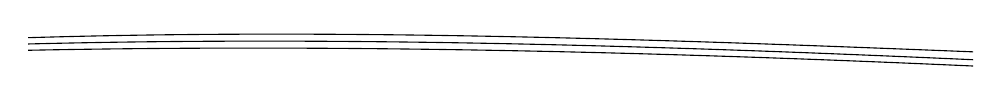
\begin{tikzpicture}
\draw (0,0) .. controls (4,.12) and (8,-.02) .. (12,-.18);
\draw (0,-.08) .. controls (4,.02) and (8,-.10) .. (12,-.28);
\draw (0,-.16) .. controls (4,-.08) and (8,-.18) .. (12,-.36);
\end{tikzpicture}}

1.

\uline{p 0}.\quad titre :\qquad $\ell'$ (minuscule)

$(1.0)\ \ell\,5$\qquad donc\qquad ?

\begingroup
\setbox0=\hbox{$\ell\,7$}
\hbox{\rlap{\begin{tikzpicture}[overlay,baseline=0pt]
\draw[gray,line width=.4pt] (\dimexpr\wd0+8pt\relax,16pt) .. controls (\dimexpr\wd0+2pt\relax,27pt) and (-21pt,10pt) .. (-14pt,-10pt) .. controls (-4pt,-24pt) and (\dimexpr\wd0+18pt\relax,-1pt) .. (\dimexpr\wd0+10pt\relax,13pt);
\draw[line width=.3pt] (-15pt,-13pt) -- (\linewidth,-13pt);
\end{tikzpicture}}\box0}
\endgroup\quad à quel concept se rapporte ``lequel''.

\smallskip

\uline{p1}\quad $\ell\,12$\quad français : choisie\quad ; ``qui est'' tend à faire croire qu'on impose une condition supplémentaire

$\ell\,16$\quad $=B$ donc le symbole est malheureux;\quad $=A'_K$ de toute façon.

\rule{\linewidth}{0.3pt}

p2.\quad $\ell\,2$\quad pourquoi \begingroup
\setbox0=\hbox{G}
\hbox{\rlap{\begin{tikzpicture}[overlay,baseline=0pt]
\draw[gray,line width=.35pt] (0pt,13pt) .. controls (-8pt,9pt) and (-5pt,-6pt) .. (3pt,-6pt) .. controls (\dimexpr\wd0+8pt\relax,-3pt) and (\dimexpr\wd0+8pt\relax,14pt) .. (\dimexpr\wd0-1pt\relax,14pt) .. controls (3pt,14pt) and (3pt,12pt) .. (2pt,11pt);
\end{tikzpicture}}\box0}
\endgroup{}roupe
\quad -- épimorphisme n'est pas la définition d'isogénie --

$\ell\,15$\quad -- supprimer séparé type fini au bénéfice du seul quasi projectif.

-- que $A\mathbin{\underset{S}{\times}}\operatorname{Spec}(K)\xrightarrow{\sim}A_K$ est une trivialité

\margin{2}

\scanpage{4}
\mspage{2}
\margin{\begin{tikzpicture}\draw (0,0)--(.6,-.65);\end{tikzpicture}}

$\ell-8$\quad pourquoi\quad \uline{donc}\qquad ?

\rule{\linewidth}{0.3pt}

p3\quad $\ell-8,-9$\qquad $B$ ?

\rule{\linewidth}{0.3pt}

p4.\quad 1.3.1.\quad As tu vérifié si l'accouplement d'A. \unsure{M|$\Pi$}. coïncide avec le tien ?

$\ell\,4$.\quad \uline{formellement} non ramifié ?

$\ell\,7$.\quad \uline{séparablement} clos ?

$\ell\,14-20$.\quad Est-ce utile à dire, en l'absence de référence à ce que ce peut vouloir dire ?

$\ell-5$\quad Qu'il soit\qquad et\qquad signifierait\qquad plutôt ?

\rule{\linewidth}{0.3pt}

pg5\quad $\ell-2$\quad français :\quad les classes $\unsure{w|\omega}$\qquad \uline{en}\qquad relatifs.

\rule{\linewidth}{0.3pt}

pg6\quad $\ell\,4$\quad français.\quad dire\quad un Module inversible simple\qquad ?

\deleted{\illegible{5}}

\figure{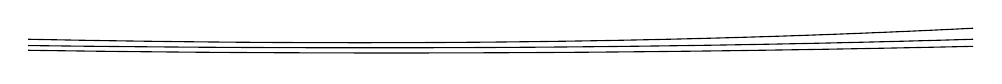
\begin{tikzpicture}\draw (0,.08).. controls (4,0) and (8,.02) .. (12,.22);\draw (0,0).. controls (4,-.05) and (8,-.04) .. (12,.08);\draw (0,-.06).. controls (4,-.12) and (8,-.10) .. (12,-.01);\end{tikzpicture}}

\reversemarginpar
\margin{\textcircled{\textcircled{2}}}
\normalmarginpar
pg7\quad français \uline{$\ell-9$}\quad \begingroup\setbox0=\hbox{$\unsure{\subset|<}$}\hbox{\rlap{\begin{tikzpicture}[overlay,baseline=0pt]\draw[gray,line width=.35pt] (1pt,13pt) .. controls (-7pt,9pt) and (-6pt,-7pt) .. (3pt,-8pt) .. controls (\dimexpr\wd0+10pt\relax,-5pt) and (\dimexpr\wd0+10pt\relax,12pt) .. (\dimexpr\wd0+2pt\relax,14pt) .. controls (6pt,15pt) and (5pt,13pt) .. (4pt,12pt);\end{tikzpicture}}\box0}\endgroup $\unsure{\dot{L}_0|i_0}$\quad donc \textcircled{c'} est

\deleted{$\ell-7$\quad \unsure{si|ni}\quad \illegible{1}\quad que}
\quad $\ell-7$\quad \begingroup\setbox0=\hbox{que}\hbox{\rlap{\begin{tikzpicture}[overlay,baseline=0pt]\draw[gray,line width=.35pt] (1pt,13pt) .. controls (-8pt,11pt) and (-8pt,-7pt) .. (6pt,-8pt) .. controls (\dimexpr\wd0+10pt\relax,-8pt) and (\dimexpr\wd0+11pt\relax,11pt) .. (\dimexpr\wd0-1pt\relax,14pt);\end{tikzpicture}}\box0}\endgroup (le $2^{\underline{\mathrm{e}}}$)

\rule{\linewidth}{0.3pt}

pg8\quad français\quad $\ell\,4$\quad par exemple\quad
$\overset{\text{\inserted{\begingroup\setbox0=\hbox{pour}\hbox{\rlap{\begin{tikzpicture}[overlay,baseline=0pt]\draw[gray,line width=.35pt] (-4pt,6pt) .. controls (-5pt,-6pt) and (\dimexpr\wd0-1pt\relax,-7pt) .. (\dimexpr\wd0+5pt\relax,-1pt) .. controls (\dimexpr\wd0+8pt\relax,10pt) and (\dimexpr\wd0-1pt\relax,13pt) .. (10pt,12pt);\draw[gray,line width=.35pt] (8pt,12pt) .. controls (1pt,14pt) and (-3pt,10pt) .. (-4pt,8pt);\end{tikzpicture}}\box0}\endgroup\,?}}}{\text{\unsure{à|k}}}$\quad $\ldots$

$\ell-7$\quad \uline{le} terme

\rule{\linewidth}{0.3pt}

pg14.\quad L'argument est un peu immoral; si $X$ et $Y$ sont extensions d'une VA par un tore et si $\varphi:X\longrightarrow Y$ est donné, alors $\varphi$ est strictement compatible à la filtration par le poids et $\varphi$ est une isogénie si et seulement si $T_\ell(\varphi)$ en est une.

\rule{\linewidth}{0.3pt}

\mbox{
\begin{tikzpicture}[overlay]\draw (.8,.08) ellipse (1.0 and .6);\end{tikzpicture}pg\deleted{\unsure{19|15|17}}20.}
\quad Rmq 2.6 a)\quad $S$ est-il un trait dans cette remarque ; sait-on assez sur le passage à la limite et Néron ?

\reversemarginpar
\margin{3}
\normalmarginpar

\scanpage{5}
\mspage{3}
\margin{\figure{\begin{tikzpicture}\draw (0,0)--(.6,-.65);\end{tikzpicture}}}

\noindent\textcircled{3}\quad
\uline{pg23}\quad On peut dire plus simplement que ${}_nK$ est étale séparé car ${}_nK=\operatorname{Ker}({}_nG\longrightarrow{}_nH)$. En a), ne dirais-tu pas que ${}_nK_{\bar s}$ est isomorphe à un sous-groupe de ${}_nK_{\bar t}$.

\noindent\uline{pg24}\quad a) $\ell\,15$ :\quad
\begingroup\setbox0=\hbox{$\dim$}\hbox{\rlap{
\begin{tikzpicture}[overlay,baseline=0pt]\draw[gray,line width=.35pt] (3pt,15pt) .. controls (-10pt,11pt) and (-7pt,-6pt) .. (8pt,-7pt) .. controls (\dimexpr\wd0+14pt\relax,-7pt) and (\dimexpr\wd0+15pt\relax,17pt) .. (\dimexpr\wd0-1pt\relax,18pt);\end{tikzpicture}}\box0}\endgroup$\operatorname{Ker}(u_\eta)=0$\quad ?

\noindent\rlap{\begin{tikzpicture}[overlay,baseline]
\draw (0.62,.65) .. controls (-.15,.63) and (-.45,.08) .. (-.22,-.54) .. controls (.04,-1.03) and (.95,-.59) .. (1.02,.11) .. controls (1.05,.47) and (.84,.68) .. (.62,.65);
\draw[gray] (-.17,.47) .. controls (-.42,.13) and (-.27,-.05) .. (.1,-.03);
\end{tikzpicture}}
\uline{pg28}\quad Les notions introduites dans 3.5 ont elles été définies pour $S$ non hensélien ? (il faudrait au moins choisir un groupe d'inertie).
\inserted{[\unsure{itou|item} pour 3.7]}

\noindent\uline{pg29}\quad $\ell-2$\quad la terminologie ``clôture normale'' est-elle encore canonique ?

\figure{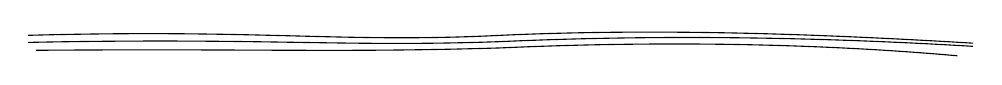
\begin{tikzpicture}
\draw (0,0) .. controls (3,.08) and (4,-.1) .. (6,0) .. controls (8,.09) and (10,.02) .. (12,-.1);
\draw (0,-.09) .. controls (3,-.03) and (4,-.15) .. (6,-.08) .. controls (8,.01) and (10,-.02) .. (12,-.14);
\draw (.1,-.19) .. controls (3,-.17) and (4,-.22) .. (6,-.16) .. controls (8,-.07) and (10,-.1) .. (11.8,-.26);
\end{tikzpicture}}

\noindent\textcircled{4}\quad
\uline{p32}\quad $\ell\,8$\quad ne dépend
\begingroup\setbox0=\hbox{pas}\hbox{\rlap{\begin{tikzpicture}[overlay,baseline=0pt]\draw[gray,line width=.35pt] (\dimexpr\wd0+2pt\relax,15pt) .. controls (-10pt,20pt) and (-8pt,-8pt) .. (3pt,-8pt) .. controls (\dimexpr\wd0+12pt\relax,-8pt) and (\dimexpr\wd0+10pt\relax,8pt) .. (\dimexpr\wd0+5pt\relax,13pt);\end{tikzpicture}}\box0}\endgroup

\noindent\rlap{\begin{tikzpicture}[overlay,baseline]
\draw (1.1,.28) .. controls (.83,.83) and (-1.0,.46) .. (-1.65,-.25) .. controls (-2,-.95) and (-1.15,-1.44) .. (-.22,-1.29) .. controls (.72,-1.15) and (1.33,-.3) .. (1.17,.2);
\end{tikzpicture}}
\makebox[0pt][r]{\raisebox{-.5ex}{\Large ?}\hspace{1.5em}}\uline{pg33 ss}\quad
(4.2)\quad Ne donnerais tu pas un énoncé style ``voisinage tubulaire'' compréhensible. La vérité est

\deleted{\illegible{1}} on a un morphisme de topos $\operatorname{Spec}(K)_{\mathrm{et}}\xrightarrow{\varphi}\operatorname{Spec}(k)_{\mathrm{et}}$ (``\unsure{ext.|ent.} du corps résiduel'') et $A_0^0$ est un schéma relatif sur $(\operatorname{Spec}(K))_{\mathrm{et}}$ annelé par $\varphi^*\mathcal O$ [le $\varphi^*$ des faisceaux d'ensembles] - Même chose d'ailleurs pour
\[
\begin{array}[t]{c}\text{lim}\\[-.8ex]\longrightarrow\\[-.6ex]\text{ramifier.}\end{array}\;A_0
\]

\noindent\rlap{\begin{tikzpicture}[overlay,baseline]\draw[rotate=23] (-.15,-.1) ellipse (1.35 and .52);\end{tikzpicture}}
\makebox[0pt][r]{\raisebox{-.8ex}{\unsure{si} ?}\hspace{1.5em}}\uline{pg36}\quad
$\ell-6$.\quad ``ce n'est pas la trace qui est contragrédiente; l'énoncé primitif était correct -

\noindent\uline{pg40}\quad (4.5.4)\quad Qu'est-il écrit dans la marge ?

$\ell-1$\quad Quel est loc cit. ?

$\ell\,3$\quad $\ell$-groupe signifie-t-il tué par $\ell$, ou par un $\ell^k$ ?

le \unsure{trait|tout} est-il strictement local ? ce serait plus agréable.

\margin{4}

\scanpage{6}
\mspage{4}
\margin{\begin{tikzpicture}\draw (0,0) .. controls (.2,-.3) and (.5,-.45) .. (.6,-.7);\end{tikzpicture}}
\reversemarginpar

\begingroup\setbox0=\hbox{\uline{pg41}}\hbox{\rlap{\begin{tikzpicture}[overlay,baseline=0pt]\draw[gray,line width=.35pt] (2pt,17pt) .. controls (-17pt,16pt) and (-16pt,-20pt) .. (6pt,-23pt) .. controls (\dimexpr\wd0+13pt\relax,-25pt) and (\dimexpr\wd0+15pt\relax,19pt) .. (13pt,23pt) .. controls (5pt,24pt) and (-5pt,19pt) .. (-7pt,15pt);\end{tikzpicture}}\box0}\endgroup{}
\quad $\ell-2$\quad ``fonction de Dirac'' est malheureux (sur un groupe, on ne voit trop si c'est\quad ou
\[
\left\{\begin{array}{l}
f(e)=1,\ 0\ \text{ailleurs}\\
f(e)=\#G,\ 0\ \text{ailleurs}
\end{array}\right.\qquad )
\]
\margin{\shortstack[l]{guillemets\\suffisent ?}}

\uline{pg42}\quad début dém. 4.7 : le \unsure{eps|ops|cps} n'est pas clair pour $n=2$, et je n'ai pas confiance en dehors du cas strictement local.

\figure{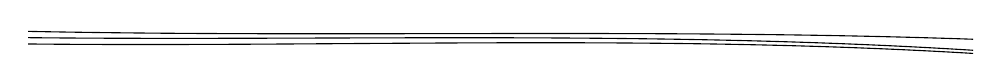
\begin{tikzpicture}\draw (0,.08).. controls (4,0) and (8,.12) .. (12,-.02);\draw (0,0).. controls (4,-.04) and (8,.09) .. (12,-.16);\draw (0,-.08).. controls (4,-.12) and (8,.04) .. (12,-.20);\end{tikzpicture}}

\margin{\begingroup\setbox0=\hbox{5}\hbox{\rlap{\begin{tikzpicture}[overlay,baseline=0pt]\draw[line width=.45pt] (5pt,17pt) .. controls (-10pt,18pt) and (-12pt,-9pt) .. (2pt,-10pt) .. controls (19pt,-12pt) and (21pt,13pt) .. (8pt,17pt);\draw[line width=.35pt] (-6pt,12pt) .. controls (-2pt,13pt) and (1pt,11pt) .. (1pt,9pt);\end{tikzpicture}}\box0}\endgroup{}}
\uline{pg\unsure{45|47}}\quad $\ell\,3$ ss\quad français : beaucoup de ``donc''.

\uline{pg46}\quad Quel est le sens de (5.2.3,1) et de \deleted{\unsure{le|la}} ``par définition'' qui suit --

S'agit-il de pro-objets, ou de schémas.
\margin{\begingroup\setbox0=\hbox{je le dis !}\hbox{\rlap{\begin{tikzpicture}[overlay,baseline=0pt]\draw[gray,line width=.35pt] (\dimexpr\wd0-1pt\relax,16pt) .. controls (-12pt,19pt) and (-10pt,-9pt) .. (6pt,-9pt) .. controls (\dimexpr\wd0+15pt\relax,-9pt) and (\dimexpr\wd0+11pt\relax,17pt) .. (\dimexpr\wd0-2pt\relax,16pt);\draw[gray,line width=.35pt] (\dimexpr\wd0+3pt\relax,13pt) .. controls (\dimexpr\wd0+10pt\relax,16pt) and (\dimexpr\wd0+10pt\relax,11pt) .. (\dimexpr\wd0+6pt\relax,9pt);\end{tikzpicture}}\box0}\endgroup{}}

\uline{pg48}\quad $\ell-4$\quad Pourquoi as-tu barré connexe ?

\deleted{\uline{pg53}\quad 5.7 est une redite pour $\ell\ne p$, et un peu idiot pour $\ell=p$.}\quad (utilisé en 5.15)

\mbox{
\begin{tikzpicture}[overlay]\draw (1.55,.08) ellipse (1.85 and .60);\end{tikzpicture}{\Large ?}\quad \uline{pg56 bis}\quad 5.15 :}
\quad tu n'a plus besoin ici de $\operatorname{car}(k)\ne\ell$

54 quater -- 5.11.\quad seraient plutôt que seront.

\uline{55 ter}\quad $\ell-10$. Il serait honnête de dire que 6.6 utilise $\operatorname{car}(K)=0$, via Tate
\margin{\begingroup\setbox0=\hbox{\shortstack[l]{C'est dit\\dans les hyp\\de 5.13}}\hbox{\rlap{\begin{tikzpicture}[overlay,baseline=0pt]\draw[gray,line width=.35pt] (-5pt,3pt) .. controls (-10pt,23pt) and (-5pt,35pt) .. (13pt,39pt) .. controls (37pt,43pt) and (\dimexpr\wd0+6pt\relax,32pt) .. (\dimexpr\wd0+8pt\relax,10pt) .. controls (\dimexpr\wd0+9pt\relax,-7pt) and (14pt,-9pt) .. (1pt,-7pt) .. controls (-4pt,-5pt) and (-5pt,0pt) .. (-5pt,3pt);\draw[line width=.45pt] (-7pt,5pt) .. controls (3cm,4pt) and (8cm,3pt) .. (12cm,7pt);\draw[line width=.35pt] (-7pt,1pt) .. controls (3cm,0pt) and (8cm,-1pt) .. (12cm,3pt);\draw[line width=.3pt] (-7pt,-4pt) .. controls (3cm,-6pt) and (8cm,-4pt) .. (12cm,-7pt);\end{tikzpicture}}\box0}\endgroup{}}



\margin{\begingroup\setbox0=\hbox{6}\hbox{\rlap{
\begin{tikzpicture}[overlay,baseline=0pt]\draw[line width=.45pt] (-3pt,15pt) .. controls (-12pt,9pt) and (-10pt,-8pt) .. (0pt,-10pt) .. controls (15pt,-11pt) and (22pt,7pt) .. (12pt,16pt) .. controls (7pt,18pt) and (-1pt,18pt) .. (-3pt,15pt) .. controls (-5pt,12pt) and (-5pt,11pt) .. (-5pt,9pt);\end{tikzpicture}}\box0}\endgroup{}}
\uline{pg57/58} : tu supposes tantôt $A^0$ $\ell$-divisible $(58,\ell-11)$, tantôt non $(57,\ell\,3)$

\uline{pg58}\quad $\ell-5$\quad
\mbox{\begin{tikzpicture}[overlay]\draw[gray,line width=.35pt] (.84,-.04) .. controls (.63,.34) and (.94,.63) .. (1.19,.55) .. controls (1.58,.41) and (1.31,-.19) .. (.93,-.13);\end{tikzpicture}$({}_{p^\infty}X)^0$}\quad \begingroup\setbox0=\hbox{?}\hbox{\rlap{\begin{tikzpicture}[overlay,baseline=0pt]\draw[line width=.45pt] (0pt,14pt) .. controls (-9pt,10pt) and (-8pt,-7pt) .. (0pt,-9pt) .. controls (16pt,-11pt) and (21pt,8pt) .. (12pt,15pt) .. controls (8pt,18pt) and (-2pt,18pt) .. (-4pt,13pt);\draw[line width=.35pt] (-4pt,13pt) .. controls (-1pt,18pt) and (2pt,19pt) .. (2pt,15pt);\end{tikzpicture}}\box0}\endgroup{}
\qquad itou plus loin --

\uline{pg\unsure{59|54}}\quad Je ne comprends rien -- Que fais-tu de la partie discrète ? --
\margin{\uline{CANULAR ?}!}

Je ne crois pas que la plus grande \deleted{\unsure{AG|VA}} sous VA ordinaire puisse se relever ($\hat{\mathrm m}$ en cas de bonne réduction).

\uline{ie}\quad 63 est faux (déformer de façon générale $E\times F$, $E$ et $F$ elliptiques, $E$ ordinaire, $F$ non ordinaire ; général $\Rightarrow$ générique simple.

\margin{5}
\normalmarginpar

\scanpage{7}
\mspage{5}
\margin{\figure{\begin{tikzpicture}\draw (0,0) .. controls (.1,-.2) and (.4,-.5) .. (.6,-.7);\end{tikzpicture}}}

\uline{pg60}\quad Je n'ai \unsure{pas|ps} confiance en ``il est immédiat'' de 6.4.
\reversemarginpar
\margin{\leavevmode\rlap{\begin{tikzpicture}[overlay,baseline=0pt]\draw[rotate around={25:(1.55,.05)}] (1.55,.05) ellipse (1.85 and .70);\end{tikzpicture}}\parbox[t]{2.2cm}{\unsure{c'est} pourtant\\trivial}}
\normalmarginpar

\uline{pg61, 61 bis} : Je n'ai \unsure{pas|ps} lu.

Il me semble qu'il doit être possible de définir, à isogénie près, des ``parties finies'' et ``parties toriques'', ayant le bon rang --
\reversemarginpar
\margin{\leavevmode\rlap{\begin{tikzpicture}[overlay,baseline=0pt]\draw (1.80,-.86) .. controls (.90,-1.32) and (-.35,-1.12) .. (-.17,-.38) .. controls (.02,.24) and (1.31,.99) .. (1.95,.58) .. controls (2.27,.34) and (2.29,-.25) .. (2.05,-.54);\draw (2.32,.95) .. controls (1.91,.24) and (1.77,-.30) .. (1.92,-.48) .. controls (1.98,-.55) and (2.05,-.59) .. (2.14,-.63);\end{tikzpicture}}\parbox[t]{2.2cm}{non, mon\\argument\\marche}}
\normalmarginpar

\uline{pg\unsure{64|68|67}/}\deleted{\unsure{bis}} : \deleted{\illegible{1}} (réf. à Serre pour \unsure{l'indép.|l'insép.} de $\ell$ ligne 11 ?)

Un peu malhonnête d'être si bref, car 6.6 est utilisé en 5.13.
\reversemarginpar
\margin{\begingroup\setbox0=\hbox{\shortstack[r]{que faire\\?}}\hbox{\rlap{\begin{tikzpicture}[overlay,baseline=0pt]\draw[gray,line width=.35pt] (-5pt,5pt) .. controls (-14pt,18pt) and (15pt,34pt) .. (\dimexpr\wd0+3pt\relax,29pt) .. controls (\dimexpr\wd0+12pt\relax,28pt) and (\dimexpr\wd0+9pt\relax,8pt) .. (\dimexpr\wd0+8pt\relax,4pt) .. controls (\dimexpr\wd0+9pt\relax,-9pt) and (10pt,-9pt) .. (-5pt,5pt);\draw[line width=.45pt] (-10pt,3pt)--(12cm,-1pt);\draw[line width=.40pt] (-10pt,-1pt)--(12cm,-5pt);\draw[line width=.30pt] (-10pt,-5pt)--(12cm,-9pt);\end{tikzpicture}}\box0}\endgroup{}}
\normalmarginpar



\reversemarginpar
\margin{\begingroup\setbox0=\hbox{7}\hbox{\rlap{
\begin{tikzpicture}[overlay,baseline=0pt]\draw[line width=.45pt] (-1pt,15pt) .. controls (-14pt,13pt) and (-12pt,-10pt) .. (1pt,-11pt) .. controls (20pt,-10pt) and (24pt,12pt) .. (12pt,18pt) .. controls (6pt,21pt) and (-2pt,17pt) .. (-1pt,15pt)--(1pt,11pt);\end{tikzpicture}}\box0}\endgroup{}}
\normalmarginpar
\uline{p65}.\quad $A_0$ n'est pas défini\margin{si}

\uline{p.67}\quad (7.1.4)\quad français --
\reversemarginpar
\margin{\begingroup\setbox0=\hbox{?}\hbox{\rlap{\begin{tikzpicture}[overlay,baseline=0pt]\draw[gray,line width=.35pt] (8pt,22pt) .. controls (-13pt,25pt) and (-13pt,-18pt) .. (0pt,-20pt) .. controls (20pt,-18pt) and (22pt,10pt) .. (14pt,20pt);\end{tikzpicture}}\box0}\endgroup{}}
\normalmarginpar

\figure{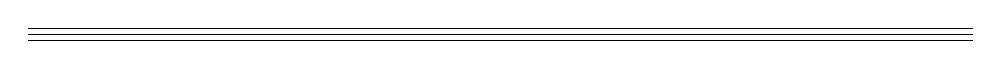
\begin{tikzpicture}\draw (0,0)--(12,0);\draw (0,-0.08)--(12,-0.08);\draw (0,-0.16)--(12,-0.16);\end{tikzpicture}}

\reversemarginpar
\margin{\begingroup\setbox0=\hbox{8}\hbox{\rlap{\begin{tikzpicture}[overlay,baseline=0pt]\draw[line width=.45pt] (10pt,19pt)--(6pt,22pt)--(-2pt,16pt) .. controls (-10pt,9pt) and (-9pt,-12pt) .. (0pt,-13pt) .. controls (12pt,-12pt) and (18pt,8pt) .. (11pt,17pt);\end{tikzpicture}}\box0}\endgroup{}}
\normalmarginpar

\figure{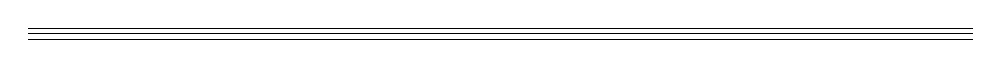
\begin{tikzpicture}\draw (0,0)--(12,0);\draw (0,-0.07)--(12,-0.07);\draw (0,-0.14)--(12,-0.14);\end{tikzpicture}}

\reversemarginpar
\margin{\begingroup\setbox0=\hbox{9}\hbox{\rlap{\begin{tikzpicture}[overlay,baseline=0pt]\draw[line width=.45pt] (3pt,17pt) .. controls (-9pt,21pt) and (-14pt,-10pt) .. (-1pt,-13pt) .. controls (14pt,-13pt) and (23pt,14pt) .. (12pt,19pt) .. controls (8pt,22pt) and (0pt,21pt) .. (3pt,17pt);\end{tikzpicture}}\box0}\endgroup{}}
\normalmarginpar
\uline{p80}\quad 9.2.3\quad $u$ plutôt que $u(q)$

\uline{p82}\quad (9.3.3)\quad $+$ compatibilité avec $R$ ? --

\uline{p87}\quad 9.4.\quad $S$ \uuline{strictement} hensélien ? (on le suppose en p88, $\ell-9$)

pas d'hyp. d'excellence ?

\uline{p91} : 9.5.8.\quad Ne \unsure{mettrait|mettrais}-tu pas une génuflexion ``au signe près''.

\uline{pg92 bis}\quad $S$ est-il strictement hensélien ?

\figure{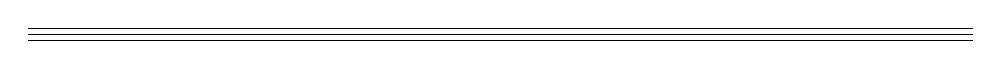
\begin{tikzpicture}\draw (0,0)--(12,0);\draw (0,-0.08)--(12,-0.08);\draw (0,-0.16)--(12,-0.16);\end{tikzpicture}}

\reversemarginpar
\margin{\begingroup\setbox0=\hbox{10}\hbox{\rlap{\begin{tikzpicture}[overlay,baseline=0pt]\draw[line width=.45pt] (2pt,18pt) .. controls (-14pt,16pt) and (-13pt,-10pt) .. (2pt,-12pt) .. controls (\dimexpr\wd0+16pt\relax,-13pt) and (\dimexpr\wd0+16pt\relax,18pt) .. (\dimexpr\wd0-1pt\relax,20pt) .. controls (5pt,22pt) and (-1pt,17pt) .. (1pt,13pt);\draw[gray,line width=.3pt] (-2pt,14pt).. controls (0pt,20pt) and (4pt,19pt) .. (5pt,17pt);\end{tikzpicture}}\box0}\endgroup{}}
\normalmarginpar
\uline{pg98}\quad 10.5.3.\quad Une extension de $K$ (qui ici est infini) est-elle requise ??.

10.5.4.\quad Dire \uline{où} on fera ces vérifications --

\reversemarginpar
\margin{6}
\normalmarginpar

\scanpage{8}
\mspage{6}
\margin{\figure{\begin{tikzpicture}\draw (0,0).. controls (.14,-.22) and (.39,-.45) .. (.5,-.65).. controls (.51,-.68) and (.52,-.72) .. (.51,-.74);\end{tikzpicture}}}

\begingroup\setbox0=\hbox{11}\hbox{\rlap{\begin{tikzpicture}[overlay,baseline=0pt]\draw[line width=.45pt] (-5pt,-6pt) .. controls (-12pt,4pt) and (-4pt,21pt) .. (8pt,22pt) .. controls (\dimexpr\wd0+9pt\relax,23pt) and (\dimexpr\wd0+12pt\relax,1pt) .. (\dimexpr\wd0+6pt\relax,-5pt) .. controls (8pt,-12pt) and (-2pt,-10pt) .. (-5pt,-6pt);\end{tikzpicture}}\box0}\endgroup{}\quad pg101\quad $\ell-6$.\quad Dire où on trouve que Néron commute à $S\mapsto\widehat S$.

\bigskip
\noindent

\begin{tikzpicture}[baseline=0pt,overlay,x=1em,y=1ex]
\draw[gray] (6.4,3.7) .. controls (7.2,2.3) and (7.8,.1) .. (7.6,-1.7)
.. controls (6.6,-3.5) and (-.6,-4.4) .. (-.7,-2.2)
.. controls (-1.2,0) and (-.2,1.7) .. (1.0,2.3)
.. controls (3.6,4.1) and (6.8,6.2) .. (6.5,3.9);
\end{tikzpicture}
\raisebox{-1.5ex}[0pt][0pt]{\makebox[0pt][l]{\textcolor{gray}{que\ \raisebox{2.3ex}{faire ?}}}}
\hspace*{3.5em}pg103\qquad Le renvoi au courage du lecteur est désagréable --

\medskip
Si j'ai bien compris, tu affirme que prolonger une \unsure{biextension} à $A\times A'$ est ``la $\hat{\mathrm m}$ chose'' que de la prolonger aux $ {}_{\ell^\infty}A\times{}_{\ell^\infty}A'$.

\margin{7}

\scanpage{28}

\diagram{\begin{tikzcd}[ampersand replacement=\&,row sep=small,column sep=small]
 \& M \arrow[dr,"{\text{\unsure{Situation|fibration}}}",shorten >=8pt] \& \& \& - \& \\
 \bullet \arrow[r,no head] \& T \arrow[r,phantom,"{\unsure{\longrightarrow|\mathord{-}}}" description] \arrow[d,phantom,"{\begin{tikzpicture}[x=1pt,y=1pt,baseline=-2pt]\draw (0,8) .. controls (3,6) and (-2,2) .. (0,0);\draw (4,8)--(4,0);\end{tikzpicture}}" description] \& G \arrow[r,no head] \& B \& 0 \arrow[l] \& \\
 \& D(M\prime) \& \& \times \& \& \unsure{\vert|1} \\
 \unsure{0|\bullet} \arrow[r,no head] \& T\prime \arrow[r,phantom,"{\unsure{\longrightarrow|\mathord{-}}}" description] \arrow[d,phantom,"{\begin{tikzpicture}[x=1pt,y=1pt,baseline=-2pt]\draw (-1,8) .. controls (2,10) and (2,7) .. (2,1)--(3,0);\draw (6,8).. controls (5,9) and (5,3) .. (5,1);\end{tikzpicture}}" description] \& G\prime \arrow[r,no head] \& B\prime \arrow[r,phantom,"{\unsure{\leftrightarrow|\rightarrow}}" description] \& 0 \& \\
 \& D(\unsure{\mu|M}) \& \& \& \& \\
 \& \unsure{\mu\prime|M\prime} \arrow[uur,"{\unsure{\beta\lambda|R\lambda}}"',pos=.2,shorten >=16pt] \& \& \& \&
\end{tikzcd}}

\margin{27}

\scanpage{29}

$\Gamma=\mathbb G$

\margin{$M\times B'\qquad\operatorname{Ext}(B',DM)$

$\deleted{\operatorname{Hom}(B',\operatorname{Ext}(\unsure{M},\unsure{\mathbb G_m}))}=0$}

\diagram{\begin{tikzcd}[ampersand replacement=\&, row sep=small,column sep=small]
B \& B'\\
M \arrow[u,"i"] \& M' \arrow[u,"i'"']
\end{tikzcd}}
\quad \unsure{une} biext.\inserted{$\mathcal E$} sous $\mathbb G_m$

\diagram{\begin{tikzcd}[ampersand replacement=\&, column sep=small]
B' \arrow[r,"\alpha'"] \& \underline{\operatorname{Ext}}(B,G_m) \arrow[r,no head] \& \underline{\operatorname{Ext}}(M\ G_m)
\end{tikzcd}}
nul\quad p.c. $\operatorname{Hom}(B',\underline{\operatorname{Ext}}(M,\overset{\substack{0\\\Vert}}{G_m}\unsure{)}$

\diagram{\begin{tikzcd}[ampersand replacement=\&, column sep=small]
B \arrow[r,no head,"\alpha"] \& \underline{\operatorname{Ext}}(B',G_m) \arrow[r,no head] \& \underline{\operatorname{Ext}}(M',G_m)
\end{tikzcd}}
nul\quad p.ex $\operatorname{Hom}(B,\underline{\operatorname{Ext}}(M',\underset{\substack{\Vert\\0}}{G_m}\unsure{)}$

d'où extensions,

\diagram{\begin{tikzcd}[ampersand replacement=\&, column sep=small,row sep=tiny]
\bullet \arrow[r,no head] \& DM \arrow[r,no head,"j'"] \arrow[d,equal] \& G' \arrow[r,no head,"p'"] \& B' \arrow[r] \& 0\\
 \& T' \& \& \&
\end{tikzcd}}

\margin{\par\noindent\rule{0.8\linewidth}{0.3pt}\par
$\mathcal E_{M,G'}$ est canoniq\textsuperscript{t}\par splitté par $\rho$
\par\noindent\rule{0.8\linewidth}{0.3pt}\par}

\diagram{\begin{tikzcd}[ampersand replacement=\&, column sep=small,row sep=tiny]
0 \arrow[r,no head] \& DM' \arrow[r,no head,"j"] \arrow[d,equal] \& G \arrow[r,no head,"p"] \& B \arrow[r] \& 0\\
 \& T \& \& \&
\end{tikzcd}}

\margin{$\mathcal E_{G,M'}$ est can.\par splitté $\rho'$
\par\noindent\rule{0.8\linewidth}{0.3pt}\par}

\uline{\unsure{Exemp}} si \deleted{\illegible{1}} $\uline{\alpha'}$ \deleted{\illegible{1}} \inserted{\unsure{est}} un isom, \unsure{alors} $i'$ \unsure{rev\textsuperscript{t}|vers} : \unsure{à} \unsure{donner|donné}

\noindent un
\diagram{\begin{tikzcd}[ampersand replacement=\&,column sep=small]
i'\in\operatorname{Hom}(M',\underline{\operatorname{Ext}}(B,G_m))
\& \operatorname{Biext}(B,M';G_m) \arrow[l,"\sim"']
\& \inserted{\operatorname{Ext}(B,D(M'))} \arrow[l,"\sim"']
\end{tikzcd}}
\noindent\hfill\deleted{\unsure{réciproq\textsuperscript{t}}}\hspace{1.3em}
\begin{flushright}
\begin{minipage}[t]{0.47\linewidth}
\begin{tikzpicture}[baseline,overlay]
\draw (0,0.65) .. controls (0,0.25) and (0,0.15) .. (0.22,0.08);
\end{tikzpicture}\hspace{0.25cm}si $\underline{\unsure{\operatorname{Ext}}}(M',\underline{\operatorname{Hom}}(B,G_m))=0$

p.ex
\makebox[0pt][l]{\begin{tikzpicture}[baseline,overlay]\draw (2.59,.36) .. controls (1.75,.51) and (.35,.44) .. (-.03,.08) .. controls (-.16,-.13) and (.77,-.29) .. (1.64,-.24) .. controls (2.34,-.18) and (2.92,-.12) .. (2.78,.23);\end{tikzpicture}}$\underline{\operatorname{Hom}}(B,G_m)=0$
\end{minipage}\hfill
\begin{minipage}[t]{0.47\linewidth}
\begin{tikzpicture}[baseline,overlay]
\draw (0,0.65) .. controls (0,0.25) and (0,0.15) .. (0.22,0.08);
\end{tikzpicture}\hspace{0.25cm}si $\operatorname{Hom}(B,\underline{\operatorname{Ext}}(M',G_m))$

$=0$\quad p.ex.

\makebox[0pt][l]{\begin{tikzpicture}[baseline,overlay]\draw (-.05,.28) .. controls (.13,.39) and (.24,.22) .. (.43,.31) .. controls (.85,.42) and (1.13,.30) .. (1.43,.34) .. controls (2.23,.42) and (2.57,.64) .. (2.76,.25) .. controls (3.12,-.21) and (2.22,-.47) .. (1.80,-.36) .. controls (1.21,-.51) and (.44,-.48) .. (.10,-.20) .. controls (.01,-.10) and (-.02,.03) .. (.02,.16);\end{tikzpicture}}$\underline{\operatorname{Ext}}(M',G_m)=0$
\end{minipage}
\end{flushright}

\unsure{aussi|ainsi} pour. \unsure{Donc} la donnée de $i'$ \unsure{équiv} : celle de l'ext. $G$. Et \unsure{réciproquement}

Considérons l'image inverse\makebox[0pt][l]{\begin{tikzpicture}[baseline,overlay]\draw (.12,-.12) .. controls (-.28,.20) and (-.17,.70) .. (.25,.75) .. controls (.75,.92) and (1.10,.65) .. (1.14,.31) .. controls (1.20,.09) and (.48,-.12) .. (.27,-.29) .. controls (.16,-.39) and (.20,-.53) .. (.26,-.61);\end{tikzpicture}}\inserted{$\mathcal E_{\unsure{i'|i},i'}$}
de $\mathcal E$ sur $(M,M')$. Alors des \unsure{splittages|splittage}\inserted{$\rho_i$} de cette biextension correspondent aux hom $j$ de $M$ dans $G$ relevant $i$, \unsure{ou aux|ou à}\,$j'$ de $M'$ dans $G'$ relev. de $i'$.

\diagram{\begin{tikzcd}[ampersand replacement=\&, row sep=tiny,column sep=small]
M \arrow[r,no head] \& G \arrow[r,no head] \& B\\
M' \arrow[r,no head] \& G' \arrow[r,no head] \& B'
\end{tikzcd}}

\makebox[0pt][l]{\begin{tikzpicture}[baseline,overlay]\draw (.01,-.12) .. controls (-.18,.13) and (-.02,.40) .. (.49,.39) .. controls (.99,.39) and (1.34,.28) .. (1.36,.09) .. controls (1.40,-.10) and (.39,-.22) .. (.14,-.18);\end{tikzpicture}}\deleted{\unsure{dans le|sur $k$}}

\deleted{\unsure{Si}} \inserted{Deux \unsure{relèv\textsuperscript{ts}|relèvements}} $j$ et $j'$ \deleted{\unsure{se}} correspond ainsi

\deleted{\unsure{les|des} \unsure{conditions} splitt. $\sigma$ canonique \deleted{\illegible{1}} $\sigma$ de $\mathcal E_{G,M'}$ et un splitt. $\sigma$ canonique $\sigma'$ de $\mathcal E_{M,G'}$, ces \unsure{deux} splitt. $\sigma$ coïncident sur $M,M'$ \unsure{avec} le splittage \unsure{donné} $h$ de $\mathcal E_{M,M'}$.}

ssi les deux splittages de $\mathcal E_{M,M'}$\unsure{)|,} \unsure{les|l'un} \unsure{déduits|déduit} d'\unsure{une|eux} par du splittage $\rho$ de $\mathcal E_{M,G'}$ \unsure{et} de $j':M'\longrightarrow G'$, d'autre par \unsure{du|un} splittage $\rho'$ de $\mathcal E_{\unsure{G|M},\unsure{M'|G'}}$ et de $j:M\mathbin{-}G$, coïncident.

\margin{28}

\scanpage{30}

or le premier membre (grâce à (2.3.2)) est $\phi^{n'}(x,my)=m\phi^{n'}(x,y)$. La compatibilité \deleted{(2.3.1)} (2.\deleted{2}3.2) \deleted{\unsure{est}}\inserted{implique} à son tour \deleted{\unsure{conséquence} de} la compatibilité symétrique\inserted{de (2.3.1)}, exprimée par la commutativité de

(2.3.\deleted{\unsure{3|5}}4)
\deleted{\illegible{1}}
\diagram{\begin{tikzcd}[ampersand replacement=\&, column sep=small,row sep=large]
{}_nP \arrow[d,"\mathrm{id}"] \& \times \& {}_{n'}Q \arrow[d,"m"] \arrow[rr,"{\phi^{n'}_\xi|_{{}_nP\times{}_{n'}Q}}"] \& \& {}_nG \arrow[d,"\mathrm{id}"]\\
 {}_nP \& \times \& {}_nQ \arrow[rr,"\phi^n_\xi"] \& \& {}_nG
\end{tikzcd}},

qui s'écrit en formules
\[
(2.3.\deleted{4}5)\qquad \phi^n(x,my)=\phi^{n'}(x,y)\qquad (x\in{}_nP(S),\ y\in{}_nQ(S)).
\]

\deleted{Montrons comment (2.3.2) implique (2.3.\unsure{4|2}). avec les notations de cette dernière formule,}
\deleted{\unsure{c}}Comme ${}_{mn'}P\xrightarrow{m}{}_nP$ est un épimorphisme, on est ramené à prouver (2.3.2) dans le cas où $x=mx'$, où $x'\in{}_{n'}P(S)$, \deleted{donc}\inserted{Or} on a
\[
\deleted{\phi^n(\unsure{mx},y)=\phi^n(m^2x',y)=\phi^n}
\quad
\phi^n_{\inserted{\xi}}(mx',my)\makebox[0pt][l]{\begin{tikzpicture}[overlay,baseline,x=1ex,y=1ex]\draw[line width=.25pt] (-1.9,2.8) .. controls (-2.3,2.1) and (-1.1,2.0) .. (-.2,1.7) -- (.55,1.1) -- (.93,-.65) -- (-1.50,-1.10);\end{tikzpicture}}\overset{\inserted{(2.3.3)}}{=}\unsure{m|n}\makebox[0pt][l]{\begin{tikzpicture}[overlay,baseline,x=1ex,y=1ex]\draw[line width=.35pt] (2.0,3.05) -- (2.05,2.55) -- (-.10,2.05) -- (-.60,1.5) -- (-.90,-1.0) -- (2.40,-1.05) -- (2.45,-1.75);\end{tikzpicture}}\phi^{n'}_{\inserted{\xi}}(x',y)=\phi^{n'}_{\inserted{\xi}}(mx',y)
\]
(par bilinéarité de $\phi^{n'}$) $=\phi^{n'}_{\inserted{\xi}}(x,y)$ puisque $x=mx'$ \deleted{\illegible{1}}dans ${}_{n'}P(S)$, ce qui établit (2.3.5).

Prouvons donc la compatibilité (2.3.1). La fonctorialité\inserted{en $Q$} de l'\unsure{homomorphisme|hmomorphisme} (2.1.2) nous montre qu'on peut supposer $nQ=0$. Alors (2.1.2) est le composé

\diagram{\begin{tikzcd}[ampersand replacement=\&, column sep=small]
\operatorname{Biext}^1(P,Q;G) \arrow[r,"\sim"] \& \operatorname{Hom}(\underline{\operatorname{Tor}}_1(P,Q),G) \& \operatorname{Hom}({}_nP\otimes Q,G) \arrow[l,"\sim"',"{\begin{tikzpicture}[x=1em,y=1em,baseline=-.3ex]\fill (0,0) -- (-.11,.10) -- (.10,.23) -- (.07,.08) -- (.19,.02) -- (.10,-.12) -- (-.08,-.10) -- cycle;\end{tikzpicture}}"{description,pos=0,inner sep=0pt,fill=none}]
\end{tikzcd}},

\deleted{en $Q$ nous montre que (2.1.2) est le composé}
\[
\deleted{\operatorname{Biext}^1(P,Q;G)\qquad\operatorname{Hom}(\operatorname{Tor}_1(P,Q),G)\qquad\operatorname{Hom}(\operatorname{Tor}_1(P,{}_nQ),G)}
\]

où la première flèche est celle de (1.1.3) et ne dépend pas du choix de $n$, et où la deuxième flèche est transposée de l'isomorphisme $\underline{\operatorname{Tor}}_1(P,Q)\overset{\inserted{\unsure{\partial|\delta}}}{\xrightarrow{\sim}}{}_nP\otimes Q$ défini dans (1.3.4). Donc la compatibilité voulue équivaut essentiellement à \deleted{celle} la commutativité du diagramme

\diagram{\begin{tikzcd}[ampersand replacement=\&, row sep=small,column sep=large]
 \& {}_{n'}P\otimes Q \arrow[dd,"m\otimes\mathrm{id}_Q"]\\
\underline{\operatorname{Tor}}_1(P,Q) \arrow[ur] \arrow[dr] \& \\
 \& {}_nP\otimes Q\quad\deleted{\unsure{4|\xi}}\quad\deleted{\unsure{\xi}}
\end{tikzcd}},

où les flèches obliques sont les deux isomorphismes du type (1.3.4), relatifs à $n$ et $n'$ respectivement. Or cette compatibilité résulte de

\margin{29}

\scanpage{31}

Supposons $j$ et $j'$ ainsi choisis. Si $j,j'$ sont injectifs, on en déduit une biextension
\inserted{\rlap{\raisebox{.4ex}{\begin{tikzpicture}[baseline]\draw (.14,-.21) .. controls (-.15,.02) and (.15,.30) .. (.86,.30) .. controls (1.57,.34) and (2.00,.19) .. (1.98,-.02) .. controls (1.88,-.19) and (.72,-.29) .. (.14,-.21) -- (.03,-.35) .. controls (-.05,-.42) and (-.02,-.49) .. (.08,-.55);\end{tikzpicture}}}canonique}
\deleted{\unsure{de|des}} $(A,A')$, où $A=G/M$, $A'=G'/M'$. Dans le cas général, posons

\deleted{\unsure{p\textsuperscript{r}|ps} \unsure{dire|dis} qu'on a une biextension de}
\[
A=\left[\underset{\text{deg.}\,\unsure{<|-}1}{M}\longrightarrow\underset{\text{deg}\,0}{G}\right],\qquad
A'=\left[M'\unsure{\longrightarrow|\mathbin{-}}G'\right].
\]

d'où
\diagram{\begin{tabular}{@{}c@{\quad}c@{\quad}c@{}}
\begin{tikzcd}[ampersand replacement=\&,row sep=small,column sep=small]
 \& \& A \arrow[dl,"1"'] \& \& \\
 \unsure{\leftarrow|\mathbin{-}} \& M \arrow[rr,"{\begin{tikzpicture}[baseline,x=1em,y=1em]\draw[line width=.4pt] (-.38,-.3)--(.38,-.3);\end{tikzpicture}}"{description,pos=.30,inner sep=0pt,fill=none}] \& \& G \arrow[ul] \arrow[r,no head] \& \phantom{0}
\end{tikzcd}
&
\begin{minipage}{2.5cm}\centering\unsure{complexe} de\par\unsure{faisceaux|chaînes} ?\end{minipage}
&
\begin{tikzcd}[ampersand replacement=\&,row sep=small,column sep=small]
 \& \& A' \arrow[dl,"1"'] \& \\
 \phantom{0} \& M' \arrow[l] \arrow[rr,no head] \& \& G' \arrow[ul]
\end{tikzcd}
\end{tabular}}

on \unsure{va|en} \unsure{définir|définit} une \deleted{\unsure{biextension}} classe canonique
\[
\xi\in\operatorname{Ext}^1(A\mathbin{\overset{L}{\otimes}}A',G_m),
\]

\margin{\unsure{pour ainsi dire|pourquoi} ?}
\noindent\llap{\raisebox{-2.65cm}[0pt][0pt]{\begin{tikzpicture}\draw (0,2.8) .. controls (-.15,1.9) and (-.2,.7) .. (0,.3) .. controls (.2,.05) and (.2,-.08) .. (.08,-.18);\end{tikzpicture}}\hspace{.7em}}%
\begin{minipage}[t][3cm][t]{\linewidth}
jouant le rôle d'une biextension de $(A,A')$ par $G_m$.

\medskip
Soit en effet \textendash\,\textendash\,\textendash\,\textemdash\,\textendash
\end{minipage}

\unsure{Soit|Soient}
\[
{}_nA\overset{\text{\unsure{dfn|def}}}{=}\deleted{\unsure{R}}\underline{\operatorname{Ext}}^0(\mathbb Z/n\mathbb Z,A),\qquad
{}_nA'=\operatorname{\underline{Ex}t}^0(\mathbb Z/n\mathbb Z,A')
\]
on trouve, \unsure{que|qu'on}, grâce aux \unsure{triangle|triangles} plus haut,
\margin{\deleted{\uline{\unsure{Soit}}}}
\[
\left\{\begin{aligned}
{}_nM&=0\quad
\overset{\text{\inserted{\rlap{\raisebox{.25ex}{\begin{tikzpicture}[baseline]\draw (.02,-.22) .. controls (-.18,.03) and (-.05,.30) .. (.35,.32) .. controls (.81,.34) and (.99,.07) .. (.82,-.13) -- (.10,-.28);\draw (.50,-.20)--(.72,-.42);\end{tikzpicture}}}\unsure{resp.|pq}}}}{\deleted{{}_nM'=0}}\\
nG&=G\quad\text{p.ex}\quad\text{\deleted{\unsure{par}}}\ nB=B,\ nT=T\quad(\text{ce dernier résulte de }{}_nM=0
\end{aligned}\right.
\]

\margin{\begin{minipage}[t]{1.85cm}donne aussi autre \unsure{interprét\textsuperscript{tion}|interpr.\textsuperscript{tion}} de $ {}_nA$, via hom. cobord si $nG=G$\end{minipage}\hspace{.15cm}\begin{tikzpicture}[baseline]\draw (0,-2.5)--(0,0);\end{tikzpicture}}
\diagram{\begin{tikzcd}[ampersand replacement=\&,column sep=small]
0 \arrow[r] \& \underset{\makebox[0pt][l]{\begin{tikzpicture}[overlay,baseline,x=1em,y=1ex]\draw (.55,1.7) .. controls (.45,2.6) and (1.45,2.2) .. (2.10,2.4) .. controls (2.32,2.45) and (2.40,3.4) .. (2.55,3.7) .. controls (2.70,2.8) and (3.15,2.1) .. (4.30,2.2) .. controls (4.8,2.3) and (5.20,2.1) .. (5.35,1.5);\end{tikzpicture}}(D(\unsure{M'_n|M_n}),\unsure{nB|{}_nB}),\,\text{si }nT=T}{ {}_nG} \arrow[r] \& {}_nA \arrow[r] \& M_n \arrow[r] \& 0
\end{tikzcd}}

et on a de $\widehat{\mathrm m}$ une suite exacte
\diagram{\begin{tikzcd}[ampersand replacement=\&,column sep=small]
0 \arrow[r] \& {}_n\unsure{G'|C'} \arrow[r] \& {}_nA' \arrow[r] \& M'_n \arrow[r] \& 0
\end{tikzcd}}

sous les hyp. duales; \unsure{passant|passons} à la limite sur $n=\ell^\nu$, \unsure{on a|on les}
\[
\vcenter{\hbox{\begin{tikzpicture}[x=1em,y=1em]\draw[line width=.45pt] (.22,2.20) .. controls (.27,1.85) and (.29,1.25) .. (.19,1.11) .. controls (-.12,1.22) and (-.10,.92) .. (.19,1.05) .. controls (.24,.80) and (.22,.30) .. (.39,0);\end{tikzpicture}}}\,\begin{gathered}
\begin{tikzcd}[ampersand replacement=\&,column sep=small]
0 \arrow[r] \& T_\ell(G) \arrow[r] \& T_\ell(A) \arrow[r] \& M\otimes\mathbb Z_\ell \arrow[r,no head] \& 0
\end{tikzcd}\\
\begin{tikzcd}[ampersand replacement=\&,column sep=small]
0 \arrow[r,no head] \& T_\ell(A') \arrow[r] \& T_\ell(A') \arrow[r,no head] \& M'\otimes\mathbb Z_\ell \arrow[r] \& 0
\end{tikzcd}
\end{gathered}
\]
\margin{30}

\scanpage{32}

\margin{\begin{minipage}{1.5cm}
\begin{tikzpicture}[overlay,baseline=0pt]
\draw (0.77,0.36) .. controls (0.74,0.78) and (0.21,0.84) .. (0.06,0.36)
 .. controls (-0.08,-0.01) and (0.07,-0.40) .. (0.38,-0.37)
 .. controls (0.65,-0.34) and (0.84,-0.05) .. (0.80,0.21);
\draw (0.94,-0.43) .. controls (1.12,-0.73) and (0.89,-1.11) .. (0.56,-1.10)
 .. controls (0.24,-1.08) and (0.12,-0.72) .. (0.32,-0.48)
 .. controls (0.49,-0.23) and (0.82,-0.22) .. (0.90,-0.46);
\end{tikzpicture}
\(\varphi^{(\ell)}\)\\[0.5em]
\hspace*{0.25cm}\({}_{\ell^\nu}P\)
\end{minipage}}
\[
(2.2.4)\qquad
\deleted{\unsure{\$}}\phi^{(\ell)}_{\inserted{\xi}}\deleted{\unsure{\$}}
=(\phi^{\ell^\nu}_{\inserted{\xi}})_{\nu\geq0},
\quad\text{où}\quad
\phi^{\ell^\nu}_{\inserted{\xi}}:{}_{\ell^\nu}P\times{}_{\ell^\nu}Q\longrightarrow G.
\]
Les diagrammes \rule{0pt}{4ex}\makebox[0pt][l]{\hspace*{-2em}\raisebox{2.4ex}{\inserted{commutatifs}}}\makebox[0pt][l]{\begin{tikzpicture}[overlay,baseline,x=1em,y=1ex]\draw (-.40,-.55) .. controls (-.72,.45) and (-.42,1.2) .. (.35,1.25) .. controls (1.8,1.6) and (3.8,1.2) .. (4.35,1.40) .. controls (5.2,1.9) and (5.35,2.7) .. (5.05,3.25);\end{tikzpicture}}\deleted{déduits} de (2.2.2) en y faisant $n=\ell^\nu$, $n'=\ell^{\nu'}$, pour $\nu'\geq\nu$, montrent que $\phi^{(\ell)}_{\inserted{\xi}}$ peut être interprété comme un accouplement de \deleted{pro-groupes} systèmes projectifs de groupes
\[
(2.2.5)\qquad
\phi^{(\ell)}_{\inserted{\xi}}:T_\ell(P)\times T_\ell(Q)\longrightarrow T_\ell(G),
\]
où, pour un \deleted{\unsure{G}}groupe $M$ de $T$ et un nombre premier $\ell$, on désigne par
\[
T_\ell(M)=({}_{\ell^\nu}M)_{\nu\geq0}
\]
le système projectif des ${}_{\ell^\nu}M$. L'accouplement \deleted{\unsure{\$}} (2.2.5) est encore appelé \uline{l'accouplement} $\ell$-\uline{adique associé à} $\xi$ (ou à la biextension $E$ de classe $\xi$). Pour $\xi$ variable, on obtient un homomorphisme canonique
\[
(2.2.6)\qquad
\operatorname{Biext}^{\inserted{1}}(P,Q;G)\longrightarrow
\operatorname{Hom}(T_\ell(P)\otimes T_\ell(Q),T_\ell(G)).
\]
On notera que les homomorphismes (2.1.2) sont \uline{fonctoriels} en $P,Q,G$
\par\noindent
\begin{tikzpicture}[overlay,baseline=0pt]
\draw (-0.78,-0.17) .. controls (-0.20,-0.24) and (0.57,-0.09) .. (1.37,-0.12) .. controls (1.43,-0.12) and (1.43,-0.08) .. (1.41,-0.03);
\draw (-0.91,-0.36) .. controls (-0.28,-0.44) and (0.78,-0.37) .. (1.57,-0.32);
\end{tikzpicture}
(pour $n$ fixé), d'où on déduit qu'il en est de même de (2.2.6).

2.3. \deleted{On peut regarder} La compatibilité (2.2.2) permet de retrouver $\phi^n_{\inserted{\xi}}$ connaissant $\phi^{n'}_{\inserted{\xi}}$, pourvu que ${}_{n'}Q\xrightarrow{m}{}_nQ$ \inserted{soit} un épimorphisme, --- \deleted{(NB l'h} condition satisfaite, comme il est bien connu, si $nQ=Q$. En effet, comme ${}_{n'}P\xrightarrow{m}{}_nP$ est aussi un épimorphisme, $\phi^n_{\inserted{\xi}}$ se déduit \deleted{\unsure{de}}alors de $\phi^{n'}_{\inserted{\xi}}$ par passage au quotient. On peut cependant \rule{0pt}{4ex}\makebox[0pt][l]{\raisebox{2.4ex}{\inserted{donner}}}\makebox[0pt][l]{\begin{tikzpicture}[overlay,baseline,x=1em,y=1ex]\draw[line width=.45pt] (-.25,-.55) -- (-.31,1.02) .. controls (-.28,1.60) and (.0,1.56) .. (.55,1.53) .. controls (1.45,1.58) and (2.60,1.22) .. (3.25,1.71) .. controls (3.65,2.0) and (3.64,2.63) .. (3.45,2.91);\draw[line width=.25pt] (-.17,-.75) .. controls (-.42,.45) and (.10,1.48) .. (.62,1.30) .. controls (1.6,1.13) and (2.90,1.03) .. (3.56,2.18);\end{tikzpicture}} une compatibilité légèrement plus précise que (2.2.2), qui permet d\deleted{e}'exprimer $\phi^n$ en termes de $\phi^{n'}$ sans aucune restriction sur $Q$, par la commutativité de

(2.3.1)
\diagram{\begin{tikzcd}[ampersand replacement=\&,column sep=small,row sep=large]
{}_{n'}P \arrow[d,"m"] \& \times \& {}_nQ \arrow[d,"\mathrm{id}"] \arrow[rr,"{\phi^{n'}_{\inserted{\xi}}|_{{}_{n'}P\times{}_nQ}}"] \& \& {}_nG \arrow[d,"\mathrm{id}"]\\
{}_{\deleted{\unsure{m|n}}n}P \& \times \& {}_nQ \arrow[rr,"\phi^n_{\inserted{\xi}}"] \& \& {}_nG
\end{tikzcd}},

en formules
\[
(2.3.2)\qquad
\phi^n_{\inserted{\xi}}(mx,y)=\phi^{n'}_{\inserted{\xi}}(x,y)
\qquad(x\in{}_{n'}P(S),\ y\in{}_nQ(S)).
\]
Cette formule implique évidemment la commutativité de (2.2.2), qui s'écrit en effet
\[
\inserted{(2.3.3)}\qquad
\phi^n_{\inserted{\xi}}(mx,my)=m\phi^{n'}_{\inserted{\xi}}(x,y)
\qquad(x\in{}_{n'}P(S),\ y\in{}_{n'}P(S)),
\]
\margin{31}

\scanpage{33}

\deleted{\unsure{Les inclusions}}

on a \uline{loc}. des hom
\[
{}_nA\unsure{\longrightarrow|\mathbin{-}} A,\qquad{}_nA'\unsure{\longrightarrow|\mathbin{-}} A'
\]
d'où \uline{loc} \unsure{des hom}
\diagram{\begin{tikzcd}[
ampersand replacement=\&,column sep=large,row sep=large,
execute at end picture={
\draw[gray,line width=0.3pt]
([xshift=-5pt,yshift=4pt]\tikzcdmatrixname-2-2.west)
-- ([xshift=-1pt,yshift=-1pt]\tikzcdmatrixname-2-2.west)
-- ([xshift=-7pt,yshift=-4pt]\tikzcdmatrixname-2-2.west);
}]
\operatorname{Ext}^1(A\mathbin{\overset{L}{\otimes}}A\unsure{'},G_m)
\arrow[r]
\arrow[dr,start anchor=south east,end anchor=west,shorten >=5pt,bend right=6,
dash pattern=on 7mm off 3mm on 40mm]
\& \operatorname{Ext}^1({}_nA\mathbin{\overset{L}{\otimes}}{}_nA',G_m)\unsure{\mathbin{-}|=}0\arrow[d]\\
\& \operatorname{Hom}({}_nA\otimes{}_nA',G_m)
\end{tikzcd}}

qui se recollent, donc \unsure{bien} définis \unsure{glob\textsuperscript{t}}\unsure{.} Donc l'\unsure{élémt} $\unsure{\xi|\zeta}$ envisagé plus haut nous donne
\[
\varphi_n^{\unsure{\xi|\zeta}}:{}_nA\otimes{}_nA'\unsure{\longrightarrow|\mathbin{-}} G_m
\]
et par passage à la limite
\[
T_\ell(A)\times T_\ell(A')\longrightarrow T_\ell(G_m)\overset{\text{def}}{=}\mathbb Z_\ell(1).
\]

\par\noindent
\begin{minipage}[t]{0.025\linewidth}
\vspace{1.2\baselineskip}
\begin{tikzpicture}[baseline=(current bounding box.north)]
\draw (0,0) .. controls (0.02,-0.55) and (0.09,-1.25) .. (0.08,-1.8);
\end{tikzpicture}
\end{minipage}%
\begin{minipage}[t]{0.965\linewidth}
\uline{Prop} Dans cet accouplement, $D(\unsure{M'_n|M_n})$ est orthogonal à ${}_nG'$, \deleted{\unsure{et}} (a un sens si ${}_nM'=0$) et \deleted{$D(M_{\unsure{n}}$} ${}_nG$ est orth. à $D(M_n)$ (a un sens si $\unsure{'}\,{}_nM=0$). Les accouplements induits
\end{minipage}

\diagram{\begin{tikzcd}[
ampersand replacement=\&,column sep=small,row sep=small,
execute at end picture={
\draw[gray,line width=0.3pt]
([xshift=-8pt,yshift=-3pt]\tikzcdmatrixname-1-2.south west)
.. controls ([xshift=-8pt,yshift=15pt]\tikzcdmatrixname-1-2.north west)
and ([xshift=10pt,yshift=15pt]\tikzcdmatrixname-1-2.north east)
.. ([xshift=10pt,yshift=-2pt]\tikzcdmatrixname-1-2.south east)
.. controls ([xshift=10pt,yshift=-12pt]\tikzcdmatrixname-2-2.south east)
and ([xshift=-12pt,yshift=-12pt]\tikzcdmatrixname-3-4.south west)
.. ([xshift=-3pt,yshift=-10pt]\tikzcdmatrixname-3-4.south);
}]
\deleted{\unsure{{}_nA/{}_n}} \& {}_nA'/{}_nG' \& \times \& D(M'_n)\arrow[rr] \& \& G_m\\
\& \unsure{\wr|\rho} \& \& \Vert \& \&\\
\& \unsure{,}\quad M'_n \& \& {}_n\unsure{T'|T} \& \&
\end{tikzcd}}

et
\diagram{\begin{tikzcd}[ampersand replacement=\&,column sep=small,row sep=small]
D(M_n) \& \times \& {}_nA/{}_nG\arrow[r,no head] \& G_m\\
\Vert \& \& \unsure{\wr|\rho} \&\\
{}_nT \& \& M_n \&
\end{tikzcd}},

ainsi que

\noindent\deleted{\unsure{et}}\quad
\begin{minipage}{0.85\linewidth}
\diagram{\begin{tikzcd}[ampersand replacement=\&,column sep=small,row sep=small]
{}_nG/{}_n\unsure{T|\Pi} \& \times \& {}_nG'/{}_nT'\\
\unsure{\Vert|\wr}\ \deleted{\unsure{{}_nT_n|{}_nT}} \& \& \unsure{\rho|\wr}\\
{}_n\unsure{\underline{B}|B} \& \& {}_nB'
\end{tikzcd}}
\end{minipage}

sont ceux qu'on devine.

\par\noindent
\begin{minipage}[t]{0.025\linewidth}
\vspace{1.2\baselineskip}
\begin{tikzpicture}[baseline=(current bounding box.north)]
\draw (0,0)--(-0.003,-0.20);
\draw (-0.004,-0.24)--(-0.006,-0.40);
\draw (-0.006,-0.44)--(-0.005,-0.49);
\draw (-0.005,-0.51) .. controls (0.02,-0.95) and (-0.02,-1.6) .. (-0.025,-2.0);
\end{tikzpicture}
\end{minipage}%
\begin{minipage}[t]{0.965\linewidth}
\uline{Corollaire} Si l'accouplement entre ${}_nB$ et ${}_nB'$ est une dualité parfaite \unsure{car|(car} $\unsure{\alpha|n}T_n=\unsure{n|\alpha}T'_n=0$) \deleted{\unsure{donc}} et si ${}_nM=0$, ${}_nM'=\unsure{0}$, $nB=B$, $\unsure{n|\mathbin{-}}B'=B'$, alors l'accouplement de ${}_nA$ et ${}_nA'$ est une dualité parfaite.
\end{minipage}
\margin{32}

\scanpage{34}

2. \uline{Accouplements définis par une biextension}.

2.1. Soit $n$ un entier $>0$, et supposons qu'on a
\[
(2.1\deleted{)}.1)\qquad nP=P.
\]
\noindent\makebox[0pt][l]{\begin{tikzpicture}[overlay,x=1em,y=1ex]
\draw (-2.7,-.40)..controls(-2.77,-.58)and(-2.75,-.69)..(-2.55,-.65)
..controls(-1.1,-.48)and(.15,-.55)..(.65,-.50);
\draw (-2.3,-1.05)..controls(-.8,-.91)and(.7,-.96)..(1.2,-.93);
\draw (1.7,-.94)..controls(1.9,-.91)and(2.1,-.96)..(2.05,-1.13);
\end{tikzpicture}}Considérons alors l'homomorphisme composé

(2.1.2)
\diagram{\begin{tikzcd}[ampersand replacement=\&,column sep=large]
\operatorname{Biext}^{\inserted{1}}(P,Q;G)
\arrow[r]\arrow[rr,bend left=20,"\varphi^n"]
\&\operatorname{Biext}^{\inserted{1}}(P,{}_nQ;G)\arrow[r,"\sim"]
\&\operatorname{Hom}({}_nP\otimes{}_nQ;G)
\end{tikzcd}},

où la première flèche est la restriction à $(P,{}_nQ)$, et la deuxième est l'isomorphisme (1.3.\deleted{5}6). Il permet, à tout élément
\makebox[0pt][l]{\begin{tikzpicture}[overlay,x=1em,y=1ex]
\draw (.10,1.2)..controls(1.2,2.05)and(9.7,2.05)..(11.55,1.15)
..controls(12.2,.5)and(12.1,-.8)..(10.9,-1.1)
..controls(6.2,-1.55)and(.7,-1.2)..(-.38,-.25)
..controls(-.52,.12)and(-.48,.66)..(-.35,.9);
\draw (-.15,1.15)..controls(2,2.25)and(10.5,2.0)..(11.8,.85)
..controls(12.45,-.1)and(11.65,-1.2)..(9.8,-1.35)
..controls(5.7,-1.55)and(.6,-1.32)..(-.35,-.55);
\draw[->](-.35,-.55)..controls(-2.9,-1.9)and(-7.8,-.95)..(-10.0,-2.25);
\end{tikzpicture}}$\xi\in\operatorname{Biext}(P,Q;G)$,

(2.1.3)

à fortiori à toute biextension
\makebox[0pt][l]{\begin{tikzpicture}[overlay,x=1em,y=1ex]
\draw (.03,2.3)..controls(-.4,3.8)and(1.0,4.0)..(1.02,2.95);
\draw (1.04,2.65)..controls(1.05,2.0)and(.57,1.7)..(.40,.6);
\draw (.40,.6)..controls(.20,1.7)and(.03,1.9)..(.03,2.3);
\end{tikzpicture}}\raisebox{1.7ex}{\inserted{$E$}}
de $(P,Q)$ par $G$, de faire correspondre un\deleted{e \unsure{forme homomorphisme}} accouplement bilinéaire
\reversemarginpar
\margin{\makebox[0pt][l]{\begin{tikzpicture}[overlay,x=1em,y=1ex]
\draw (.72,1.75)..controls(-.7,2.35)and(-1.2,-1.3)..(-.15,-2.0)
..controls(1.35,-2.35)and(1.65,.75)..(1.02,1.45);
\end{tikzpicture}}$\varphi$}
\normalmarginpar
\[
(2.1.4)\qquad
\phi_{\inserted{\xi}}\text{ ou }\phi^n_{\inserted{\xi}}:{}_nP\times{}_nQ\longrightarrow G,
\]
qu'on appelle l'accouplement \uline{associé à} $\xi$ (ou à la biextension $E$).

2.2. Soit $\deleted{\unsure{ni|n'}}$ $n'$ un multiple de $n$,
\[
n'=mn,
\]
et supposons qu'on ait la relation (plus forte que (2.1.1))
\[
(2.2.1)\qquad n'P=P\quad\text{i.e.}\quad mnP=P,
\]
d'où comme en (2.1.4), pour toute $\xi\in\operatorname{Biext}(P,Q;G)$, un\deleted{e} accouplement
\[
\phi^{n'}_{\inserted{\xi}}:{}_{n'}P\times{}_{n'}Q\longrightarrow G.
\]
\deleted{Les relations entre cet accouplement et}\inserted{Il est lié à} l'accouplement $\phi^n_{\inserted{\xi}}$ \deleted{est donné} par la commutativité du diagramme suivant (\deleted{qu'on laisse au lecteur le soin d'établir).}\inserted{cf. 2.3 ci-dessous pour une démonstration):}

(2.2.2)
\diagram{\begin{tikzcd}[ampersand replacement=\&,column sep=small,row sep=large]
{}_{n'}P\arrow[d,"m"']
\&\times
\&{}_{n'\deleted{\unsure{n}}}Q\deleted{\unsure{Q}}\arrow[d,"m"]\arrow[rr,"\phi^{n'}_{\inserted{\xi}}"]
\&\&{}_{n'}G\arrow[d,"m"]\\
\deleted{\unsure{P|Q}}{}_nP
\&\deleted{\times}\times
\&{}_nQ\arrow[rr,"\phi^n_{\inserted{\xi}}"]
\&\&{}_nG
\end{tikzcd}},
\noindent\makebox[\linewidth][l]{\small
\makebox[0pt][l]{\begin{tikzpicture}[overlay,x=\linewidth,y=1ex]
\draw (-.01,-2.0)..controls(-.02,-.2)and(.025,.1)..(.12,-.35)
..controls(.38,-.70)and(.78,-.52)..(.96,-.45)
..controls(1.055,-.35)and(1.06,2.5)..(.98,2.6)
..controls(.94,2.5)and(.89,2.35)..(.85,2.2);
\end{tikzpicture}}
\inserted{où les flèches verticales sont induites par la multiplication par $m=n'/n$.}}

Notons maintenant que moyennant (2.1.1), on peut prendre pour $n'$ n'importe quelle puissance de $n$. En particulier, soit
\makebox[0pt][l]{\begin{tikzpicture}[overlay,x=1em,y=1ex]
\draw (.55,2.7)..controls(-.15,3.7)and(-.8,-1.8)..(-.45,-2.4)
..controls(.20,-3.0)and(1.2,-1.7)..(1.03,1.9);
\end{tikzpicture}}$\ell$
un nombre premier, et supposons que\deleted{\illegible{1}} l'on ait
\reversemarginpar
\margin{\makebox[0pt][l]{\begin{tikzpicture}[overlay,x=1em,y=1ex]
\draw (.75,2.1)..controls(.35,3.1)and(-.85,.4)..(-.55,-1.75)
..controls(-.35,-3.3)and(1.4,-2.2)..(1.6,.5)
..controls(1.7,1.4)and(1.45,2.1)..(1.10,2.35);
\end{tikzpicture}}$\ell$}
\normalmarginpar
\[
(2.2.3)\qquad
\makebox[0pt][l]{\begin{tikzpicture}[overlay,x=1em,y=1ex]
\draw (.55,2.5)..controls(-.25,2.9)and(-1.0,-1.7)..(-.65,-2.35)
..controls(.0,-2.65)and(1.0,.4)..(.82,1.8);
\end{tikzpicture}}\ell P=P,
\]
et considérons le système des accouplements
\margin{33}

\scanpage{35}
\begin{flushright}
P\uline{icard et dualité}
\end{flushright}
\margin{34}

\scanpage{36}
\begingroup
\setlength{\tabcolsep}{0pt}
\setbox0=\hbox{%
\begin{tabular}{@{}l@{\hspace{1em}}l@{\hspace{1em}}l@{}}
\parbox[t][21em][t]{30em}{%
\(H^0(X,\zeta_\ell)=U_\ell\)\par\vspace{3em}
\(\begin{aligned}
H^2(X,\mathbb Z/\ell)&=H^2(X,\zeta_\ell)\otimes_{\mathbb Z/\ell}\operatorname{Hom}(U_\ell,\mathbb Z/\ell)\\[1em]
&=\unsure{\mathbb Z|\zeta}_\ell\otimes_{\mathbb Z/\ell}\operatorname{Hom}(U_\ell,\mathbb Z/\ell)\\[1em]
&\simeq\deleted{\mathbb Z/\ell}\operatorname{Hom}(U_\ell,\mathbb Z/\ell)
\end{aligned}\)}
&
\parbox[t][21em][t]{40em}{%
\(H^1(X,\zeta_\ell)=P^{(\ell)}\)\quad\unsure{élémts|élts} de la jacobienne\par
\hspace*{15em}$P$ de $X$\unsure{,|.} annulés par $\ell$\par\vspace{2.3em}
\(\begin{aligned}
H^1(X,\mathbb Z/\ell)&=H^1(X,\zeta_\ell)\otimes_{\mathbb Z/\ell}\operatorname{Hom}(\unsure{U|\zeta}_\ell,\mathbb Z/\ell)\\[.6em]
&\deleted{=P^{(\ell)}\otimes}\quad\overset{\text{''}\quad}{\deleted{\operatorname{Hom}(\zeta_\ell,H}}\\[.6em]
&=P^{(\ell)}\otimes_{\mathbb Z/\ell}\operatorname{Hom}(\unsure{U|\zeta}_\ell,\mathbb Z/\ell)
\end{aligned}\)\par\vspace{1em}
\hspace*{3em}Or\quad\(P^{(\ell)}\times P^{(\ell)}\longrightarrow U_\ell\)\quad\unsure{en vertu}\par\vspace{.5em}
\hspace*{6em}%
\begingroup
\setbox2=\hbox{\strut de\hspace{1.4em}\begin{tabular}[t]{@{}l@{}}
l'autodualité de $P$ \textendash\,\textendash\,\textendash\\
\uline{et} la dualité de Kummer-Serre \textendash
\end{tabular}\hspace{.5em}}
\dimen2=\dimexpr\ht2+\dp2\relax
\rlap{\raisebox{-\dp2}{\begin{tikzpicture}[x=\wd2,y=\dimen2,baseline=0pt]
\useasboundingbox (0,0) rectangle (1,1);
\draw[line width=.3pt] (.135,1.09) .. controls (.42,1.16) and (.82,1.13) .. (.98,1.07) -- (.995,1.00);
\draw[line width=.3pt] (.12,.94) -- (.125,-.10);
\draw[line width=.3pt] (-.01,.79) -- (-.005,-.05) -- (.125,-.10) .. controls (.53,-.07) and (.82,-.03) .. (.99,-.02);
\draw[line width=.3pt] (1.00,.77) -- (1.00,.08);
\end{tikzpicture}}}\box2
\endgroup}
&
\parbox[t][21em][t]{27em}{%
\(H^2(X,\zeta_\ell)\simeq\mathbb Z/\ell\)\par\vspace{3.3em}
\(H^0(X,\mathbb Z/\ell)\simeq\mathbb Z/\ell\)}
\\
\parbox[t][12.8em][t]{30em}{%
\vspace*{1em}\(H^0(X,\zeta_p)=0\)\par\vspace{3em}
\(H^2(X,\mathbb Z/p)\simeq H^2(X,\mathbb Z/p)\simeq0\)}
&
\parbox[t][12.8em][t]{40em}{%
\vspace*{1em}\hspace*{3.5em}\(H^1(X,\zeta_p)=P^{(p)}\ =\)\quad\unsure{élémts|élts} d'ordre $p$\par
\hspace*{16em}de la jacobienne\par\vspace{1.8em}
\hspace*{3.5em}\(H^1(X,\mathbb Z/p)\simeq\)\unsure{élémts|élts} de \(H^1(X,\underline{\mathrm O}_X)\) fixes\par
\hspace*{23em}par $F$\par\vspace{.7em}
\hspace*{7em}%
\begingroup
\setbox2=\hbox{\hspace{.6em}\strut dualité de Serre - Cartier\hspace{.6em}}
\dimen2=\dimexpr\ht2+\dp2\relax
\rlap{\raisebox{-\dp2}{\begin{tikzpicture}[x=\wd2,y=\dimen2,baseline=0pt]
\useasboundingbox (0,0) rectangle (1,1);
\draw[line width=.3pt] (.025,1.27) -- (.17,1.25);
\draw[line width=.3pt] (.185,1.25) .. controls (.50,1.23) and (.80,1.32) .. (1.00,1.36);
\draw[line width=.3pt] (0,1.02) -- (0,-.23) .. controls (.25,-.28) and (.75,-.13) .. (1.00,-.11);
\draw[line width=.3pt] (1.00,1.08) -- (1.00,.02);
\end{tikzpicture}}}\box2
\endgroup}
&
\parbox[t][12.8em][t]{27em}{%
\vspace*{.6em}\(H^2(X,\zeta_p)\simeq\mathbb Z/p\)\par\vspace{3.5em}
\(H^0(X,\mathbb Z/p)\simeq\mathbb Z/p\)}
\\
\parbox[t][5.4em][t]{30em}{\vspace*{1.3em}\(H^0(X,i_p)=0\)}
&
\parbox[t][5.4em][t]{40em}{\vspace*{1.3em}\hspace*{8em}%
\(H^1(X,\unsure{i}_p)\simeq{}_F H^1(X,\underline{\mathrm O}_X)\)%
\raisebox{1.7ex}{\begin{tikzpicture}[x=.25ex,y=.25ex]\fill (0,3)--(1.2,4.2)--(2.8,5.1)--(4.2,5)--(4.8,4.6)--(6.4,5.3)--(6.5,4.6)--(5.6,3.8)--(5.9,2.8)--(5.2,1.5)--(3.7,0)--(3.3,.8)--(2.8,.1)--(2.2,.8)--(1.1,.7)--(1.2,2.7)--cycle;\end{tikzpicture}}}
&
\parbox[t][5.4em][t]{27em}{\vspace*{1.3em}\(H^2(X,i_p)=H^1(X,\underline{\mathrm O}_X)_F\)}
\end{tabular}}
\dimen0=\dimexpr\ht0+\dp0\relax
\noindent\resizebox{\linewidth}{!}{\hspace*{15em}%
\llap{\raisebox{\dimexpr.45\dimen0-\dp0\relax}{\rotatebox{90}{Cohomologie discrète}}\hspace{12.7em}}%
\llap{\raisebox{\dimexpr.37\dimen0-\dp0\relax}{\begin{tikzpicture}[x=1ex,y=1ex]\draw (0.8,4)--(0.9,1.5); \draw (0.7,1.5)--(2.3,1.8); \draw (1,2.4)--(0.8,0.8); \draw (0.7,1.6)--(2.1,1.1); \draw (3.8,4)..controls (3.4,4) and (3,3.9)..(3,3.6)..controls (3,2.5) and (3,1.3)..(3.4,0.6);\end{tikzpicture}}\hspace{12.7em}}%
\rlap{\raisebox{-\dp0}{\begin{tikzpicture}[x=\wd0,y=\dimen0,baseline=0pt]
\useasboundingbox (0,0) rectangle (1,1);
\draw[line width=.3pt] (.307,1.025) .. controls (.305,.83) and (.308,.67) .. (.309,.48) -- (.310,.425);
\draw[line width=.3pt] (.310,.419) -- (.312,.285);
\draw[line width=.3pt] (.312,.279) -- (.312,.14) .. controls (.312,.08) and (.315,.02) .. (.318,-.025);
\draw[line width=.3pt] (.720,1.025) .. controls (.723,.82) and (.720,.65) .. (.722,.523);
\draw[line width=.3pt] (.724,.520) .. controls (.722,.51) and (.725,.50) .. (.724,.480);
\draw[line width=.3pt] (.725,.464) .. controls (.727,.42) and (.723,.38) .. (.726,.350)
-- (.728,.343) -- (.725,.337) .. controls (.727,.30) and (.727,.28) .. (.725,.267)
.. controls (.724,.256) and (.727,.253) .. (.726,.246)
.. controls (.729,.21) and (.729,.17) .. (.726,.14)
.. controls (.724,.11) and (.726,.09) .. (.730,.09) -- (.733,.086) -- (.731,.080)
.. controls (.728,.05) and (.731,.015) .. (.734,-.025);
\draw[line width=.3pt] (.729,-.270)--(.735,-.282);
\draw[line width=.3pt] (-.12,.464) .. controls (.20,.463) and (.52,.471) .. (.72,.462) .. controls (.86,.459) and (.98,.462) .. (1.01,.474);
\draw[line width=.3pt] (-.12,.138) .. controls (.06,.137) and (.23,.142) .. (.305,.141);
\draw[line width=.3pt] (.322,.141) .. controls (.51,.147) and (.63,.142) .. (.72,.139) .. controls (.88,.139) and (.98,.142) .. (1.01,.139);
\draw[line width=.3pt] (-.075,.925) .. controls (-.085,.93) and (-.086,.79) .. (-.082,.65)
.. controls (-.078,.57) and (-.093,.515) .. (-.112,.50)
.. controls (-.087,.478) and (-.078,.44) .. (-.079,.35)
.. controls (-.083,.25) and (-.086,.18) .. (-.075,.155);
\end{tikzpicture}}}\box0}
\endgroup
\margin{35}

\scanpage{37}
\[
H^{\unsure{1|n}}\bigl(X,\underbrace{\underline{\operatorname{Ext}}^{\unsure{1|n}}(f^*(B),G_{mX}})\bigr)
\]
\margin{\begin{tikzpicture}[x=1mm,y=1mm] \fill (0,4) ellipse (.12 and .17); \draw[line width=.3pt] (-.2,0) .. controls (.5,.05) and (.8,-.5) .. (.8,-1.2); \end{tikzpicture}}
\diagram{\begin{tikzcd}[ampersand replacement=\&,column sep=small,row sep=large,execute at end picture={
\path (\tikzcdmatrixname-2-1.north) -- (\tikzcdmatrixname-1-1.south)
 coordinate[pos=.15] (doublebase) coordinate[pos=.9] (doubletop);
\draw ([xshift=-.07cm]doublebase) .. controls ([xshift=-.12cm,yshift=.18cm]doublebase) and ([xshift=-.08cm,yshift=-.15cm]doubletop) .. ([xshift=-.07cm]doubletop);
\draw ([xshift=.04cm,yshift=.1cm]doublebase) .. controls ([xshift=.16cm,yshift=.09cm]doublebase) and ([xshift=.07cm,yshift=.17cm]doublebase) .. ([xshift=.07cm,yshift=.25cm]doublebase) -- ([xshift=.07cm,yshift=-.01cm]doubletop);
\draw ([xshift=-.10cm,yshift=-.13cm]doubletop) -- ([xshift=.05cm,yshift=.035cm]doubletop) -- ([xshift=.26cm,yshift=-.09cm]doubletop);
}]
\operatorname{Ext}_X(\overset{A}{\overset{\begin{tikzpicture}[baseline]\draw (0,0) .. controls (.25,.08) and (.55,.04) .. (.8,-.14);\end{tikzpicture}}{\unsure{f^*(B)|f_!(B)}}},G_{mX})
 \& {}\simeq\operatorname{Ext}_{\unsure{S|s}}(B,f_!(G_{mX}))\\
H^p(X,\underline{\operatorname{Ext}}^q_X(A,G_{mX})) \&
\end{tikzcd}}

\figure{\begin{tikzpicture}\draw (0,.12) .. controls (3,.25) and (6,.22) .. (10,0);\end{tikzpicture}}

\noindent\llap{\raisebox{-5.7cm}[0pt][0pt]{\begin{tikzpicture}[x=1cm,y=1cm]
\draw (0,5.65) .. controls (-.12,5.8) and (-.08,5.25) .. (-.06,4.9)
 .. controls (-.02,4.6) and (-.03,4.25) .. (-.17,4.17)
 .. controls (-.45,4.38) and (-.24,3.98) .. (-.13,4.08)
 .. controls (.02,3.85) and (.12,2.5) .. (.18,1.85)
 .. controls (.23,1.1) and (.24,.3) .. (.7,0);
\draw (.14,2.13) .. controls (.18,1.94) and (.2,1.84) .. (.31,1.79);
\draw (.27,.84)--(.52,.58);
\end{tikzpicture}}\hspace{.7em}}%
\begin{minipage}{\linewidth}
\unsure{Suites|Suite} \unsure{exactes|exacte} de Cohomologie. Critère de \unsure{rationalité};

\medskip
\unsure{Fibrés universels|Fibré universel}

\medskip
Dualité de \unsure{Cartier} [\unsure{voir} \unsure{Pic|Ric} \textendash\ \textendash\ \textendash]

\medskip
Th. \unsure{projectivité} \unsure{des|du} V.A. (Th. de \unsure{rigidité})

\medskip
Propriétés \unsure{fonctorielles|finicielles} des \unsure{groupes} \textendash\ \textendash\ \textemdash

\medskip
Propriétés différentielles. des \unsure{gpes|groupes} et fibrés

\medskip
Cas \unsure{particuliers}: \begingroup\setbox0=\hbox{fibrés linéaires,}\leavevmode
\rlap{\raisebox{-.45ex}{\begin{tikzpicture}[x=\wd0,y=1ex,baseline=0pt]
\draw (.025,0) .. controls (.35,.03) and (.8,.13) .. (1.09,.18);
\draw (.25,-.55) .. controls (.45,-.63) and (.75,-.35) .. (.97,-.38);
\end{tikzpicture}}}\box0\endgroup symplectiques, orthogonaux etc \textendash\ \textemdash\ \textendash
\end{minipage}

\medskip
\unsure{Sans} doute \unsure{par|pour} une \unsure{représentation|organisation} \unsure{lin.} de \unsure{gpes|groupes} ??

\figure{\begin{tikzpicture}\draw (0,0) .. controls (2,-.05) and (3.5,.14) .. (5,.07) .. controls (7.5,.02) and (8.5,.17) .. (10,.1);\end{tikzpicture}}
\[
\deleted{\underline{\operatorname{Hom}}(G_a,G_m)}
\]
\[
\mathbb Z.\quad\mathrel{\begin{tikzpicture}[x=1ex,y=1ex,baseline=.3ex]
\draw (.38,1.45) .. controls (.21,1.08) and (.03,.28) .. (.04,.02)
 .. controls (.08,-.18) and (.19,.22) .. (.34,.34)
 .. controls (.55,.21) and (.95,.3) .. (1.15,.34)
 .. controls (1.36,.4) and (1.56,.31) .. (1.66,.18);
\draw[line width=.6pt] (.35,.35) .. controls (.76,.2) and (1.15,.43) .. (1.53,.27);
\end{tikzpicture}}\quad\mathbb Z
\]
\margin{36}

\scanpage{38}

\begin{center}-- 98 --\end{center}
\margin{n\textsuperscript{o} 316}

un automorphisme de $E$.

Si en outre $E$ est une algèbre (non nécessairement associative), et si $u$ est une dérivation (nilpotente) de $E$, alors $e^u$ est un automorphisme de \uline{l'algèbre} $E$. En effet, si $x,y\in E$, on a
\[
u^p(xy)=\sum_{r+s=p}\binom{p}{r}u^r(x)u^s(y)
\]
pour tout entier $p\geqslant0$ (formule de Leibniz). Il en résulte que :
\[
\begin{aligned}
e^u(xy)&=\sum_{p\geqslant0}\frac{1}{p!}u^p(xy)=\sum_{p\geqslant0}\sum_{r+s=p}\frac{u^r(x)}{r!}\frac{u^s(y)}{s!}\\
&=\sum_{r,s=0}^\infty\frac{u^r(x)}{r!}\frac{u^s(y)}{s!}=e^u(x)e^u(y)
\end{aligned}
\]
d'où notre assertion.

Soit maintenant $\mathfrak g$ une algèbre de Lie. Si $x$ appartient au radical nilpotent de $\mathfrak g$, la dérivation $\operatorname{ad}_{\mathfrak g}x$ de $\mathfrak g$ est nilpotente. On peut donc poser la définition suivante :

\uline{Définition} 5 -- \uline{On appelle automorphisme spécial de} $\mathfrak g$ \uline{un automorphisme de} $\mathfrak g$ \uline{de la forme} $e^{\operatorname{ad}x}$, \uline{où} $x$ e\uline{st dans le radical nilpotent de} $\mathfrak g$.

Il est clair qu'un automorphisme spécial laisse stable tout idéal de $\mathfrak g$.

\uline{Définition} 6 -- \uline{Soient} $\mathfrak g$ \uline{une algèbre de Lie}, $\unsure{\mathfrak r|r}$ \uline{son radical}. \uline{On appelle sous-algèbre de Levi de} $\mathfrak g$ \uline{toute sous-algèbre supplémentaire de} $\unsure{\mathfrak r|r}$ \uline{dans} $\mathfrak g$.

Une sous-algèbre de Levi est isomorphe à $\mathfrak g/\unsure{\mathfrak r|r}$, donc semi-simple. Comme une sous-algèbre semi-simple n'a que $0$ en commun avec $\unsure{\mathfrak r|r}$, toute sous-algèbre semi-simple $\unsure{\mathfrak h|h}$ telle que $\mathfrak g=\unsure{\mathfrak r|r}+\unsure{\mathfrak h|h}$ est une sous-algèbre de Levi ; par conséquent, l'image d'une sous-algèbre de Levi par un homomorphisme surjectif est une sous-algèbre de Levi.
\margin{37}

\scanpage{39}

$X$ propre et simple sur $k$ [\unsure{généraliser|généralisons} à une base quelconque]

$A$ V.A. sur $k$

$H^1(X,A)=\underset{n}{\varinjlim}\ {}_nH^1(X,A)$ \begin{tikzpicture}[x=1ex,y=1ex,baseline=0pt]
\fill (0,.35)--(.03,.53)--(.23,.59)--(.27,.72)--(.41,.66)--(.48,.7)--(.55,.62)--(.78,.58)--(.92,.46)--(.95,.23)--(.87,.25)--(.84,.36)--(.64,.38)--(.35,.36)--cycle;
\fill (.14,.04) ellipse (.055 and .05);
\end{tikzpicture} d'autre part on a une suite exacte
\diagram{\begin{tikzcd}[ampersand replacement=\&, column sep=small]
0 \arrow[r] \& \operatorname{Hom}(X,A)_n \arrow[r] \& {}_{\deleted{\unsure{n}}}H^1(X,{}_nA) \arrow[r] \& {}_nH^1(X,A) \arrow[r] \& 0
\end{tikzcd}}
qui s'écrit aussi
\diagram{\begin{tikzcd}[ampersand replacement=\&, column sep=small]
0 \arrow[r] \& \operatorname{Hom}(\operatorname{Alb}_X,A)_n \arrow[r] \& \operatorname{Hom}(D({}_nA),\operatorname{Pic}_X) \arrow[r] \& {}_nH^1(X,A) \arrow[r] \& 0
\end{tikzcd}}

\unsure{en effet}, cela par
\par\noindent\hspace*{0.51\linewidth}$\unsure{l|1}$
\[
\operatorname{Hom}(\operatorname{Alb}_X,A)\simeq\operatorname{Hom}(A',(\operatorname{Alb}_X)')=\operatorname{Hom}(A',\operatorname{Pic}_X^0)
\]
\[
D({}_nA)\simeq{}_nA'
\]
une suite exacte

$(*)$
\diagram{\begin{tikzcd}[ampersand replacement=\&, column sep=small]
0 \arrow[r] \& \operatorname{Hom}(A',\operatorname{Pic}_X^{\unsure{0|\tau}})_n \arrow[r] \& \operatorname{Hom}({}_{\unsure{n}}A',\operatorname{Pic}_X) \arrow[r] \& {}_nH^1(X,A) \arrow[r] \& 0
\end{tikzcd}}
et passant à la limite
\begin{tabular}[b]{@{}l@{}}
\hspace{0.3em}\inserted{\unsure{inductive}}\\[0.5ex]
\rlap{\begin{tikzpicture}[x=1em,y=1ex,baseline=0pt,overlay]
\draw[->,line width=0.35pt] (-0.2,-0.4) .. controls (-0.3,1.6) and (0.8,1.8) .. (2.1,1.8) .. controls (3.8,1.6) and (4.6,1.7) .. (5.1,2.3);
\end{tikzpicture}}sur $n$ :
\end{tabular}
\diagram{\begin{tikzcd}[ampersand replacement=\&, column sep=small,
execute at end picture={
\draw[line width=0.35pt] ([xshift=-0.6em,yshift=0.8ex]\tikzcdmatrixname.north west) -- ([xshift=0.25em,yshift=1.7ex]\tikzcdmatrixname.north east) .. controls ([xshift=.38em,yshift=1.7ex]\tikzcdmatrixname.north east) and ([xshift=.45em,yshift=1.55ex]\tikzcdmatrixname.north east) .. ([xshift=.5em,yshift=1.55ex]\tikzcdmatrixname.north east);
\draw[line width=0.35pt] ([xshift=-0.6em,yshift=-0.1ex]\tikzcdmatrixname.north west) -- ([xshift=-0.5em,yshift=-0.7ex]\tikzcdmatrixname.south west) -- ([xshift=0.3em,yshift=0ex]\tikzcdmatrixname.south east) .. controls ([xshift=.4em,yshift=0ex]\tikzcdmatrixname.south east) and ([xshift=.46em,yshift=.08ex]\tikzcdmatrixname.south east) .. ([xshift=.5em,yshift=.12ex]\tikzcdmatrixname.south east);
}]
0 \arrow[r] \& \operatorname{Hom}(A',\underline{\operatorname{Pic}}_X^{\unsure{0|\tau}})\otimes_{\mathbb Z}\mathbb Q \arrow[r] \& \operatorname{Hom}(T_{\cdot}(A'),\underline{\operatorname{Pic}}_X) \arrow[r] \& H^1(X,A) \arrow[r] \& 0
\end{tikzcd}}

Or la suite exacte $(*)$ se compare à la suite exacte déduite de
\diagram{\begin{tikzcd}[ampersand replacement=\&, column sep=small]
0 \arrow[r,no head] \& {}_n\unsure{A|\Lambda}' \arrow[r,no head] \& A' \arrow[r] \& A' \arrow[r] \& 0
\end{tikzcd}}
en appliquant $\deleted{\operatorname{Ext}^{\unsure{1}}}\underline{\operatorname{Hom}}(-,\operatorname{Pic}_X)$, on \unsure{trouve}

$(*\unsure{*|+})$
\diagram{\begin{tikzcd}[ampersand replacement=\&, column sep=small]
0 \arrow[r,no head] \& \operatorname{Hom}(A',\underline{\operatorname{Pic}}_X)_n \arrow[r] \& \operatorname{Hom}({}_{\unsure{n}}A',\underline{\operatorname{Pic}}_X) \arrow[r] \& {}_n\operatorname{Ext}^1(A',\underline{\operatorname{Pic}}_X^{\unsure{\tau|2}}) \arrow[r] \& 0
\end{tikzcd}}
qui donne à la limite
\diagram{\begin{tikzcd}[ampersand replacement=\&, column sep=small,row sep=tiny,
execute at end picture={
\draw[line width=0.35pt] ([xshift=-0.6em,yshift=0.8ex]\tikzcdmatrixname.north west) -- ([xshift=0.25em,yshift=1.2ex]\tikzcdmatrixname.north east) .. controls ([xshift=.4em,yshift=1.2ex]\tikzcdmatrixname.north east) and ([xshift=.46em,yshift=1.08ex]\tikzcdmatrixname.north east) .. ([xshift=.5em,yshift=1.04ex]\tikzcdmatrixname.north east);
\draw[line width=0.35pt] ([xshift=-0.6em,yshift=-0.1ex]\tikzcdmatrixname.north west) -- ([xshift=-0.6em,yshift=-0.6ex]\tikzcdmatrixname.south west) -- ([xshift=0.5em,yshift=-0.7ex]\tikzcdmatrixname.south east);
}]
0 \arrow[r,no head] \& \operatorname{Hom}(A',\operatorname{Pic}_X)\otimes_{\mathbb Z}\mathbb Q \arrow[r] \& \operatorname{Hom}(T_{\cdot}(A'),\operatorname{Pic}_X) \arrow[r,no head] \& \operatorname{Ext}^1(A',\underline{\operatorname{Pic}}_X) \arrow[dr,bend left=15] \& \\
 \& \& \& \& \unsure{0}
\end{tikzcd}}
\margin{38}

\scanpage{40}

On en conclut un isom canonique
\reversemarginpar
\margin{Cet isomorphisme\\
reste-t-il valable\\
pour $X$ singulier ???\\
Il est possible\\
qu'on ait\\
besoin de\\
$H^i(X,G_m)=0$\\
pour $i\geqslant2$, qui\\
\unsure{doit} tenir \unsure{si|de}\\
$X$ non sing ??}
\normalmarginpar
\begingroup
\setbox0=\hbox{$\displaystyle H^1(X,A)\xleftarrow{\sim}\operatorname{Ext}^1(A',\underline{\operatorname{Pic}}_X)$}
\ht0=\dimexpr\ht0+9pt\relax
\dp0=\dimexpr\dp0+9pt\relax
\begin{center}
\leavevmode
\rlap{\begin{tikzpicture}[overlay,baseline=0pt]
\draw (-3pt,\ht0) -- (\dimexpr\wd0+3pt\relax,\dimexpr\ht0+1pt\relax);
\draw (-7pt,\dimexpr\ht0-4pt\relax) -- (-7pt,-\dp0) -- (\dimexpr\wd0+4pt\relax,-\dp0) -- (\dimexpr\wd0+3pt\relax,\dimexpr-\dp0+2pt\relax);
\draw (\dimexpr\wd0+7pt\relax,\dimexpr\ht0-4pt\relax) -- (\dimexpr\wd0+7pt\relax,\dimexpr-\dp0+4pt\relax) -- (\dimexpr\wd0+6pt\relax,\dimexpr-\dp0+5pt\relax);
\end{tikzpicture}}
\usebox0
\end{center}
\endgroup

($A$, variété abelienne), qu'on comparera à la
formule de dualité
\begingroup
\setbox0=\hbox{$\displaystyle H^1(X,G)\simeq\operatorname{Hom}(D(G),\underline{\operatorname{Pic}}_X)$}
\ht0=\dimexpr\ht0+9pt\relax
\dp0=\dimexpr\dp0+9pt\relax
\begin{center}
\leavevmode
\rlap{\begin{tikzpicture}[overlay,baseline=0pt]
\draw (-3pt,\ht0) -- (\dimexpr\wd0+9pt\relax,\dimexpr\ht0+1pt\relax);
\draw (-7pt,\dimexpr\ht0-6pt\relax) -- (-7pt,\dimexpr-\dp0+5pt\relax);
\draw (-9pt,-\dp0) -- (\dimexpr\wd0+3pt\relax,\dimexpr-\dp0+2pt\relax) -- (\dimexpr\wd0+3pt\relax,\dimexpr-\dp0+3pt\relax);
\draw (\dimexpr\wd0+7pt\relax,\dimexpr\ht0-12pt\relax) -- (\dimexpr\wd0+7pt\relax,\dimexpr-\dp0+5pt\relax);
\end{tikzpicture}}
\usebox0
\end{center}
\endgroup
pour $G$ commutatif \unsure{affine|ffine}.

Remarque, On a des hom canoniques
\diagram{\begin{tikzcd}[ampersand replacement=\&,column sep=large,row sep=large]
\operatorname{Ext}^1(\underline{\operatorname{Alb}}_X,A) \arrow[r] \arrow[d,"\wr"] \& H^1(X,A)\\
\operatorname{Ext}^1(A',\underline{\operatorname{Alb}}_X') \arrow[d,"\unsure{\wr}"] \&\\
\operatorname{Ext}^1(A',\underline{\operatorname{Pic}}^\tau) \&
\end{tikzcd}}

dont on voit que c'est des \uline{isomorphismes}
d\uline{onc}, qui définissent sur les \unsure{trois} groupes
en question l'isomorphisme envisagé plus haut.
\reversemarginpar
\margin{39}
\normalmarginpar

\scanpage{41}

\noindent
\begin{minipage}[c]{0.10\linewidth}
\diagram{\begin{tikzcd}[ampersand replacement=\&]
X\arrow[d]\\
S
\end{tikzcd}}
\end{minipage}\hfill
\begin{minipage}[c]{0.87\linewidth}
\vspace{1em}
\[
\tikz[remember picture,overlay]\coordinate (p41-first-a) at (0,0);
\quad
\underline{\mathcal H}^{1}(X/S;\underline{\operatorname{Hom}}_{S-gr}(\gamma,G))
\xrightarrow{\sim}
\underline{\operatorname{Hom}}_{S-gr}(\gamma,\underline{\mathcal H}^{1}(X/S;G))
\quad
\tikz[remember picture,overlay]\coordinate (p41-first-b) at (0,0);
\begin{tikzpicture}[remember picture,overlay]
\draw ([yshift=2.2em]p41-first-a)--([yshift=2.2em]p41-first-b);
\draw ([xshift=8pt,yshift=-1.7em]p41-first-a)--([yshift=-1.7em]p41-first-b);
\draw ([xshift=3pt,yshift=1.5em]p41-first-a)--([xshift=3pt,yshift=-1em]p41-first-a);
\end{tikzpicture}
\]
\vspace{1em}
\end{minipage}

\begin{flushright}
isom de foncteurs, \deleted{\unsure{pour}} quand\\
tout est \uline{affine} sur $S$ (?)
\end{flushright}

\vspace{1em}
\[
\tikz[remember picture,overlay]\coordinate (p41-second-a) at (0,0);
\quad
\underline{\mathcal H}^{1}(X/S;\underline{\operatorname{Ext}}^{1}_{S-gr}(\gamma,G))
\simeq\underline{\operatorname{Ext}}^{1}_{S-gr}(\gamma,\mathcal H^{1}(X/S;G))
\quad
\tikz[remember picture,overlay]\coordinate (p41-second-b) at (0,0);
\begin{tikzpicture}[remember picture,overlay]
\draw ([xshift=3pt,yshift=2.2em]p41-second-a)--([xshift=-8pt,yshift=2.2em]p41-second-b);
\draw ([xshift=8pt,yshift=-1.7em]p41-second-a)--([yshift=-1.7em]p41-second-b);
\draw ([yshift=1.8em]p41-second-a)--([yshift=-1.3em]p41-second-a);
\draw ([yshift=2em]p41-second-b)--([yshift=-1.5em]p41-second-b);
\end{tikzpicture}
\]
\vspace{1em}

\begin{flushright}
Sous quelles conditions ???
\end{flushright}

\[
\unsure{P_X|p_X|\rho_X}
\]

\diagram{\begin{tikzcd}[ampersand replacement=\&, column sep=large]
X\arrow[d,no head,to path={(\tikztostart.south) -- ([yshift=1pt]\tikztotarget.north) .. controls ([yshift=.2pt]\tikztotarget.north) and ([xshift=-.5pt]\tikztotarget.north) .. ([xshift=-1pt]\tikztotarget.north)\tikztonodes}]\&\deleted{\gamma_X}\&\deleted{\unsure{\gamma_X\times\gamma_X}}\\
S\&\gamma\&\gamma\times\gamma
\end{tikzcd}}

\[
\mathcal H^1(X/S,\underline{\operatorname{Hom}}_{S-gr}(\gamma,G))\longrightarrow
\operatorname{Hom}(\gamma,\mathcal H^1(X/S,G))
\]

\[
\mathcal H^1(X,\operatorname{Hom}(A;B))\simeq
\]

\margin{$\deleted{\unsure{\operatorname{Ext}(A,B)|\operatorname{Ext}(X,B)}}$}

\diagram{\begin{tikzcd}[
ampersand replacement=\&,
row sep=large,
column 1/.style={nodes={anchor=west}},
execute at end picture={
\draw ([xshift=-5pt,yshift=5pt]\tikzcdmatrixname.north west)--([xshift=12.5mm,yshift=5pt]\tikzcdmatrixname.north east) .. controls ([xshift=12.8mm,yshift=5pt]\tikzcdmatrixname.north east) and ([xshift=13mm,yshift=4.8pt]\tikzcdmatrixname.north east) .. ([xshift=13mm,yshift=4pt]\tikzcdmatrixname.north east);
\draw ([xshift=-5pt,yshift=-5pt]\tikzcdmatrixname.south west)--([xshift=13mm,yshift=-5pt]\tikzcdmatrixname.south east);
\draw ([xshift=-5pt,yshift=2pt]\tikzcdmatrixname.north west)--([xshift=-5pt,yshift=-5pt]\tikzcdmatrixname.south west);
\draw ([xshift=5pt,yshift=5pt]\tikzcdmatrixname.north east)--([xshift=5pt,yshift=-5pt]\tikzcdmatrixname.south east);
}]
H^1(X/S;\underline{\operatorname{Hom}}_{S-gr}(\gamma,G))
\arrow[d,start anchor=south west,end anchor=north west,xshift=1.2em]\\
\underline{\operatorname{Hom}}_{S-gr}(\gamma,H^1(X/S;G))
\end{tikzcd}}

\margin{40}

\scanpage{42}
\margin{41}
\begingroup
\newsavebox{\scanXLIIbox}
\newlength{\scanXLIIheight}
\begin{lrbox}{\scanXLIIbox}
\begin{minipage}{\linewidth}
\footnotesize
\noindent
\begin{minipage}[t]{.25\linewidth}
\vspace{0pt}
\begin{tikzcd}[ampersand replacement=\&,column sep=1.1em,row sep=3.1em,
  execute at end picture={
    \draw[line width=.25pt]
      ([xshift=3pt]\tikzcdmatrixname-2-1.north east)
      .. controls ([xshift=15pt,yshift=12pt]\tikzcdmatrixname-2-1.north east)
      and ([xshift=5pt,yshift=-18pt]\tikzcdmatrixname-1-1.south east)
      .. ([xshift=5pt,yshift=-6pt]\tikzcdmatrixname-1-1.south east);
    \coordinate (scanXLIIpatch) at ([xshift=5pt,yshift=-8pt]\tikzcdmatrixname-1-1.south east);
    \draw[line width=.55pt]
      ([xshift=-2pt,yshift=2pt]scanXLIIpatch) -- ([xshift=-1pt,yshift=4pt]scanXLIIpatch)
      -- ([xshift=1pt,yshift=4.2pt]scanXLIIpatch) -- ([xshift=-.5pt,yshift=1pt]scanXLIIpatch)
      -- ([xshift=2pt,yshift=3pt]scanXLIIpatch) -- ([xshift=3pt,yshift=1.3pt]scanXLIIpatch)
      -- ([xshift=1pt,yshift=2pt]scanXLIIpatch) -- ([xshift=2pt,yshift=-1pt]scanXLIIpatch)
      -- ([xshift=.4pt,yshift=-2pt]scanXLIIpatch) -- ([xshift=2.5pt,yshift=-2.5pt]scanXLIIpatch);
    \draw[line width=.35pt]
      ([xshift=1pt,yshift=2pt]scanXLIIpatch) .. controls ([xshift=-1pt,yshift=-1pt]scanXLIIpatch)
      and ([xshift=2pt,yshift=-2pt]scanXLIIpatch) .. ([xshift=2pt,yshift=-.5pt]scanXLIIpatch);
    \draw[line width=.3pt]
      ([xshift=3pt]\tikzcdmatrixname-2-1.north east)
      .. controls ([xshift=7pt,yshift=4pt]\tikzcdmatrixname-2-1.north east)
      and ([xshift=8pt,yshift=12pt]\tikzcdmatrixname-2-1.north east)
      .. ([xshift=6pt,yshift=11pt]\tikzcdmatrixname-2-1.north east)
      .. controls ([xshift=3pt,yshift=8pt]\tikzcdmatrixname-2-1.north east)
      and ([xshift=6pt,yshift=4pt]\tikzcdmatrixname-2-1.north east)
      .. ([xshift=3pt]\tikzcdmatrixname-2-1.north east);
  }]
f^{-1}(U)\arrow[rr,hook,"i"]\arrow[d,"f"]\&\&X\arrow[d,"f"]\\
U\arrow[urr,"g"']\&\underset{j}{\unsure{\rightarrow|\mathbin{-}}}\&Y
\end{tikzcd}
\par\medskip
\[
\begin{gathered}
gf=i\\[.7em]
fg=j
\end{gathered}
\]
\end{minipage}\hfill
\begin{minipage}[t]{.72\linewidth}
\vspace{2.3ex}
$f$ morphisme birationnel
\makebox[0pt][l]{\raisebox{2.0ex}{\inserted{propre}}}%
\begin{tikzpicture}[overlay,baseline=0pt]
\draw[line width=.3pt] (.1em,.4ex) .. controls (.2em,1.8ex) and (.3em,2ex) .. (.9em,2.1ex);
\end{tikzpicture}%
de \unsure{préschémas} intègres $X,Y$\\[1.0ex]
$U$ ouvert de $Y$ sur lequel $f^{-1}$ est défini\\[.7ex]
\hspace*{.12\linewidth}[Si $Y$ est régulier en codim 1, \unsure{alors}\\[.7ex]
\hspace*{.16\linewidth}$U$ est le \unsure{complémentaire} d'un \unsure{ens}\\[.7ex]
\hspace*{.19\linewidth}de codim $\geqslant2$], \deleted{i.e. \unsure{ici|aussi} le \unsure{ft|$f$}}\\[.7ex]
\hspace*{.04\linewidth}i.e. on sait \unsure{$f^{-}$|qu'} \unsure{expr|existe} un voisinage $V$\\[.7ex]
\hspace*{.04\linewidth}tel que $f$ \unsure{induise} un \unsure{isom} $f^{-1}(U)\unsure{\rightarrow|\mathbin{-}}V$.
\end{minipage}
\par\bigskip\medskip
\noindent\hspace*{.12\linewidth}%
\begin{minipage}{.88\linewidth}
Soit $\xi\in\operatorname{Pic}(X)$ défini par un\hspace{.4em}%
\makebox[0pt][l]{\raisebox{3.2ex}{\hspace{.6em}\inserted{\uline{cycle}}}}%
\begin{tikzpicture}[overlay,baseline=0pt]
\draw[line width=.35pt] (-.25em,3.7ex) .. controls (.1em,2.9ex) and (.1em,1.0ex) .. (.25em,-.4ex)
  .. controls (.35em,1.5ex) and (2.4em,2.4ex) .. (3.5em,3.2ex);
\end{tikzpicture}%
\hspace{.4em}\uline{divisoriel} $\unsure{D|\Delta}$ ($X$ \unsure{connexe|normal})\\[1.2ex]
considérons \deleted{\illegible{1}} \deleted{le morphisme} $g^{-1}(\unsure{\eta|\xi})\in\operatorname{Pic}(U)$, il\\[1.0ex]
correspond à un cycle divisoriel
\end{minipage}
\end{minipage}
\end{lrbox}
\setlength{\scanXLIIheight}{\dimexpr\ht\scanXLIIbox+\dp\scanXLIIbox\relax}
\noindent\usebox{\scanXLIIbox}\kern-\wd\scanXLIIbox
\raisebox{-\dp\scanXLIIbox}[0pt][0pt]{%
\begin{tikzpicture}[x=\wd\scanXLIIbox,y=\scanXLIIheight,baseline=0pt]
\path[use as bounding box] (0,0) rectangle (1,1);
\draw[line width=.35pt] (.355,1.04) -- (.035,.43);
\draw[line width=.4pt] (.705,.98) -- (.245,.005);
\draw[line width=.35pt] (.855,.655) .. controls (.885,.615) and (.85,.57) .. (.81,.52) -- (.718,.35);
\draw[line width=.2pt] (.716,.346) -- (.683,.29) (.679,.283) -- (.639,.215)
  (.635,.208) -- (.598,.145) (.594,.138) -- (.55,.062) (.546,.055) .. controls (.532,.031) and (.521,.013) .. (.520,-.004);
\end{tikzpicture}}
\par
\endgroup

\scanpage{43}

\noindent
\begin{tabular}{@{}c@{\qquad\qquad}l@{}}
$\mathcal H^1(X;A)$ & $\operatorname{Ext}^1(A,\operatorname{Pic})$\\[-1mm]
\begin{tikzpicture}[x=1cm,y=1cm]
\draw (0,.55) .. controls (-.03,.34) and (.03,.12) .. (.07,0);
\end{tikzpicture} &\\[-1mm]
\unsure{pt singuliers|pt singulier} &
\end{tabular}

\[
\begingroup
\setbox0=\hbox{$\displaystyle\mathcal H^1(X,G)\simeq\operatorname{Hom}(D(G),\operatorname{\underline{Pi}c}_X)$}
\hbox{\rlap{\begin{tikzpicture}[overlay,baseline=0pt]
\draw (-8pt,24pt) -- (\dimexpr\wd0-16pt\relax,22pt) -- (\dimexpr\wd0-19pt\relax,20pt);
\draw (-6pt,17pt) -- (-5pt,-12pt) -- (\dimexpr\wd0+8pt\relax,-11pt) -- (\dimexpr\wd0+9pt\relax,-8pt);
\draw (\dimexpr\wd0+12pt\relax,16pt) -- (\dimexpr\wd0+10pt\relax,-5pt) -- (\dimexpr\wd0+7pt\relax,-6pt);
\end{tikzpicture}}\box0}
\endgroup
\]

\figure{\begin{tikzpicture}[x=1cm,y=1cm]
\draw[line width=.65pt] (1.14,1.40) .. controls (.52,1.58) and (-.49,.80) .. (-.05,.14)
.. controls (.37,-.42) and (1.40,.59) .. (1.14,1.40);
\draw[line width=.25pt] (-.03,.57) .. controls (.20,1.43) and (.89,1.61) .. (.99,1.25);
\fill (1.14,1.40) circle (.04);
\draw (.50,.79) .. controls (.49,.73) and (.56,.71) .. (.61,.73) .. controls (.66,.76) and (.70,.72) .. (.75,.74);
\draw[line width=.2pt] (1.22,1.11) .. controls (1.32,.63) and (.63,-.14) .. (.21,-.10);
\draw[line width=.65pt] (2.07,.38) .. controls (2.30,.85) and (2.54,1.25) .. (2.78,1.45);
\draw[line width=.55pt] (2.78,1.45) .. controls (3.32,1.81) and (3.49,.28) .. (2.95,.18);
\draw[line width=.25pt] (2.95,.18) .. controls (2.52,.13) and (2.50,1.08) .. (2.78,1.45);
\draw[line width=.65pt] (2.78,1.45) .. controls (2.93,1.77) and (3.15,1.99) .. (3.33,2.10);
\draw[line width=.25pt] (3.13,1.99) -- (3.12,1.91);
\fill (2.78,1.45) circle (.04);
\end{tikzpicture}}

\[
\mathcal H^i(X,D(G))\simeq\operatorname{Ext}^i(G,\underline{\operatorname{Pic}}_X)
\]

\[
\operatorname{Ext}^i_X(f^!(G),G_m,)\simeq
\operatorname{Ext}^i_Y(G,f_{\unsure{!|\cdot}}(G_m))
\]

\reversemarginpar
\margin{\begin{tikzcd}[ampersand replacement=\&,column sep=small,row sep=0pt]
\&X\\
f\&\unsure{\vert|\downarrow}\\
\&Y
\end{tikzcd}}
\normalmarginpar
\[
\begingroup
\setbox0=\hbox{$\displaystyle
\underline{\operatorname{Ext}}^i_X(f^*(G_{\bullet}),H^{\bullet})\simeq
\underline{\operatorname{Ext}}^i_Y(G_{\bullet},f_!(H^{\bullet}))$}
\hbox{\rlap{\begin{tikzpicture}[overlay,baseline=0pt]
\draw (-8pt,25pt) -- (\dimexpr\wd0+7pt\relax,24pt);
\draw (-7pt,21pt) -- (-6pt,-13pt) -- (\dimexpr\wd0+7pt\relax,-12pt);
\draw (-6pt,-13pt) -- (-3pt,-10pt);
\draw (\dimexpr\wd0+12pt\relax,17pt) -- (\dimexpr\wd0+11pt\relax,-8pt) -- (\dimexpr\wd0+8pt\relax,-7.5pt);
\end{tikzpicture}}\box0}
\endgroup
\]

\[H=G_m\]

\[
\underline{\operatorname{Ext}}^i_X
\bigl(\underset{\substack{\uparrow\\[-.4ex]\inserted{R}}}{f^*}(G),G_m\bigr)
\simeq\underline{\operatorname{Ext}}^i_Y\bigl(G,
\overset{\text{les \unsure{supérieurs}}}{
\begingroup
\setbox0=\hbox{$\displaystyle\underline{\operatorname{Pic}}^{\bullet}_{X/Y}$}
\hbox{\rlap{\begin{tikzpicture}[overlay,baseline=0pt]
\draw (-5pt,9pt) .. controls (0pt,22pt) and (\dimexpr\wd0+12pt\relax,22pt) .. (\dimexpr\wd0+11pt\relax,3pt)
.. controls (\dimexpr\wd0+12pt\relax,-19pt) and (-10pt,-21pt) .. (-6pt,-2pt);
\draw (20pt,-8pt) -- (20pt,-27pt);
\draw (23pt,-11pt) -- (23pt,-30pt);
\end{tikzpicture}}\box0\kern10pt}
\endgroup}
\bigr)
\]

\noindent\hspace*{.27\linewidth}
$\deleted{H^{\unsure{i}}(X,}$
\hspace{1.2cm}
\raisebox{1.5ex}[0pt][0pt]{\begin{tikzpicture}[overlay,baseline=0pt]
\draw (0pt,9pt) .. controls (0pt,-8pt) and (1pt,-19pt) .. (6pt,-27pt);
\draw (4pt,10pt) .. controls (3pt,-9pt) and (4pt,-27pt) .. (5pt,-31pt) -- (2pt,-31pt);
\end{tikzpicture}}
\par\medskip

\[
\begingroup
\setbox0=\hbox{$\displaystyle G\ \text{\uline{\unsure{affine|fini}}},\ \text{alors}\quad
H^i(X,D(G))\Longleftarrow
\deleted{\unsure{\mathcal H|E}}\operatorname{Ext}^{\unsure{p|1|i}}(G,\operatorname{Pic}^{\unsure{(q)|(1)}}_{X/Y})$}
\hbox{\rlap{\begin{tikzpicture}[overlay,baseline=0pt]
\draw (-9pt,24pt) -- (\dimexpr\wd0+12pt\relax,25pt);
\draw (-6pt,14pt) .. controls (-8pt,-5pt) and (-5pt,-13pt) .. (9pt,-13pt)
-- (\dimexpr\wd0+12pt\relax,-12pt);
\end{tikzpicture}}\box0}
\endgroup
\]

\[
\begin{array}{rll}
i=0&H^0(X,D(G))=&\deleted{\operatorname{Hom}}D(G)\\
i=1&H^1(X,D(G))=&\deleted{\unsure{\operatorname{Ex}}}\operatorname{Hom}(G,\operatorname{Pic}^{(1)})\\
i=2&H^2\unsure{(}X,D(G))\mathrel{\substack{\unsure{\#|\neq}\\\hphantom{\#}!}}&
\operatorname{Ext}^1(G,\operatorname{Pic}^{(1)}_{X/Y})+
\operatorname{Hom}(G,\operatorname{\underline{P}ic}^{\unsure{(2}}_X
\end{array}
\]

\figure{\begin{tikzpicture}[x=1cm,y=1cm]
\draw (0,.15) .. controls (3,-.1) and (6,-.1) .. (8,0);
\end{tikzpicture}}

\noindent $G$ \unsure{abélien}\unsure{,} \unsure{alors|dans} $\unsure{\mathcal A|\deleted{H}|H}$
\[
H^{i-1}(X,G')\Longleftarrow
\operatorname{Ext}^{p}_{\unsure{\mathcal A|q}}(G,\operatorname{Pic}^{\unsure{q|1|?}}_{X/Y})
\]

\[
\begin{array}{rl}
i\unsure{=}0&0=0\\
i=1&H^0(X,G')=
\end{array}
\]
\margin{42}
